\documentclass[a4paper,12pt]{article}
\newtheorem{thm}{Theorem}
\setlength{\oddsidemargin}{0.25in}
\setlength{\textwidth}{6in}
\setlength{\topmargin}{-0.25in}
\setlength{\headheight}{0.3in}
\setlength{\headsep}{0.2in}
\setlength{\textheight}{9in}
%\setlength{\footskip}{0.1in}
\usepackage{multirow}
\usepackage{fullpage}
\usepackage{graphicx}
\usepackage{amsthm}
\usepackage{amssymb}
\usepackage{url}
\usepackage{amsfonts}
\usepackage{algpseudocode}
\usepackage{mathtools}
\newcommand{\quotes}[1]{``#1''}

\usepackage{hyperref}
\hypersetup{
    colorlinks=true,
    linkcolor=blue,
    filecolor=magenta,      
    urlcolor=blue,
}


% ===== ===== ===== ===== ===== % 
% New commands set by Chuck Jia
% ===== ===== ===== ===== ===== % 

\newcommand{\code}[1]{\texttt{#1}}
\newcommand{\qnum}[1]{\noindent\textcolor{blue}{\textbf{(#1)}}}
\newcommand{\ds}{\displaystyle}
\newcommand{\sep}{\begin{center}\textcolor{gray}{\rule{\textwidth}{0.75pt}}\end{center}}
\usepackage{minted}
\usepackage{color}
\usepackage{xcolor}
\definecolor{myorange}{RGB}{255, 165, 0}
\definecolor{mydarkgreen}{RGB}{0, 100, 0}
\definecolor{mybrickred}{RGB}{132, 31, 39}
\newcommand{\km}{$k$-means }


\begin{document}\title{Homework 2\\ Applied Machine Learning \\ Fall 2017\\ CSCI-P 556/INFO-I 526}         % Enter your title between curly braces
  \author{Chuck Jia\\ jiac@indiana.edu}       % Enter your name between curly braces       % Enter your name between curly braces
\date{\today}          % Enter your date or \today between curly braces
\maketitle
\quotes{All the work herein is solely mine.}
\makeatother     % `@' is restored as a "non-letter" character
\pagestyle{plain}


 %%%%%%%%%%%%%%%%%%%%%%%%%%%%%%%%%%%%%%%%%%%%%%%%%%%%%

%     PROBLEM 1

 %%%%%%%%%%%%%%%%%%%%%%%%%%%%%%%%%%%%%%%%%%%%%%%%%%%%%

\begin{center}
\rule{\textwidth}{2pt}
\end{center}
 
\section*{Problem 1 [20 points]} 

From textbook,  Chapter 10 exercise 2 (Page 414).
\sep 

\qnum{a}
\begin{center}
  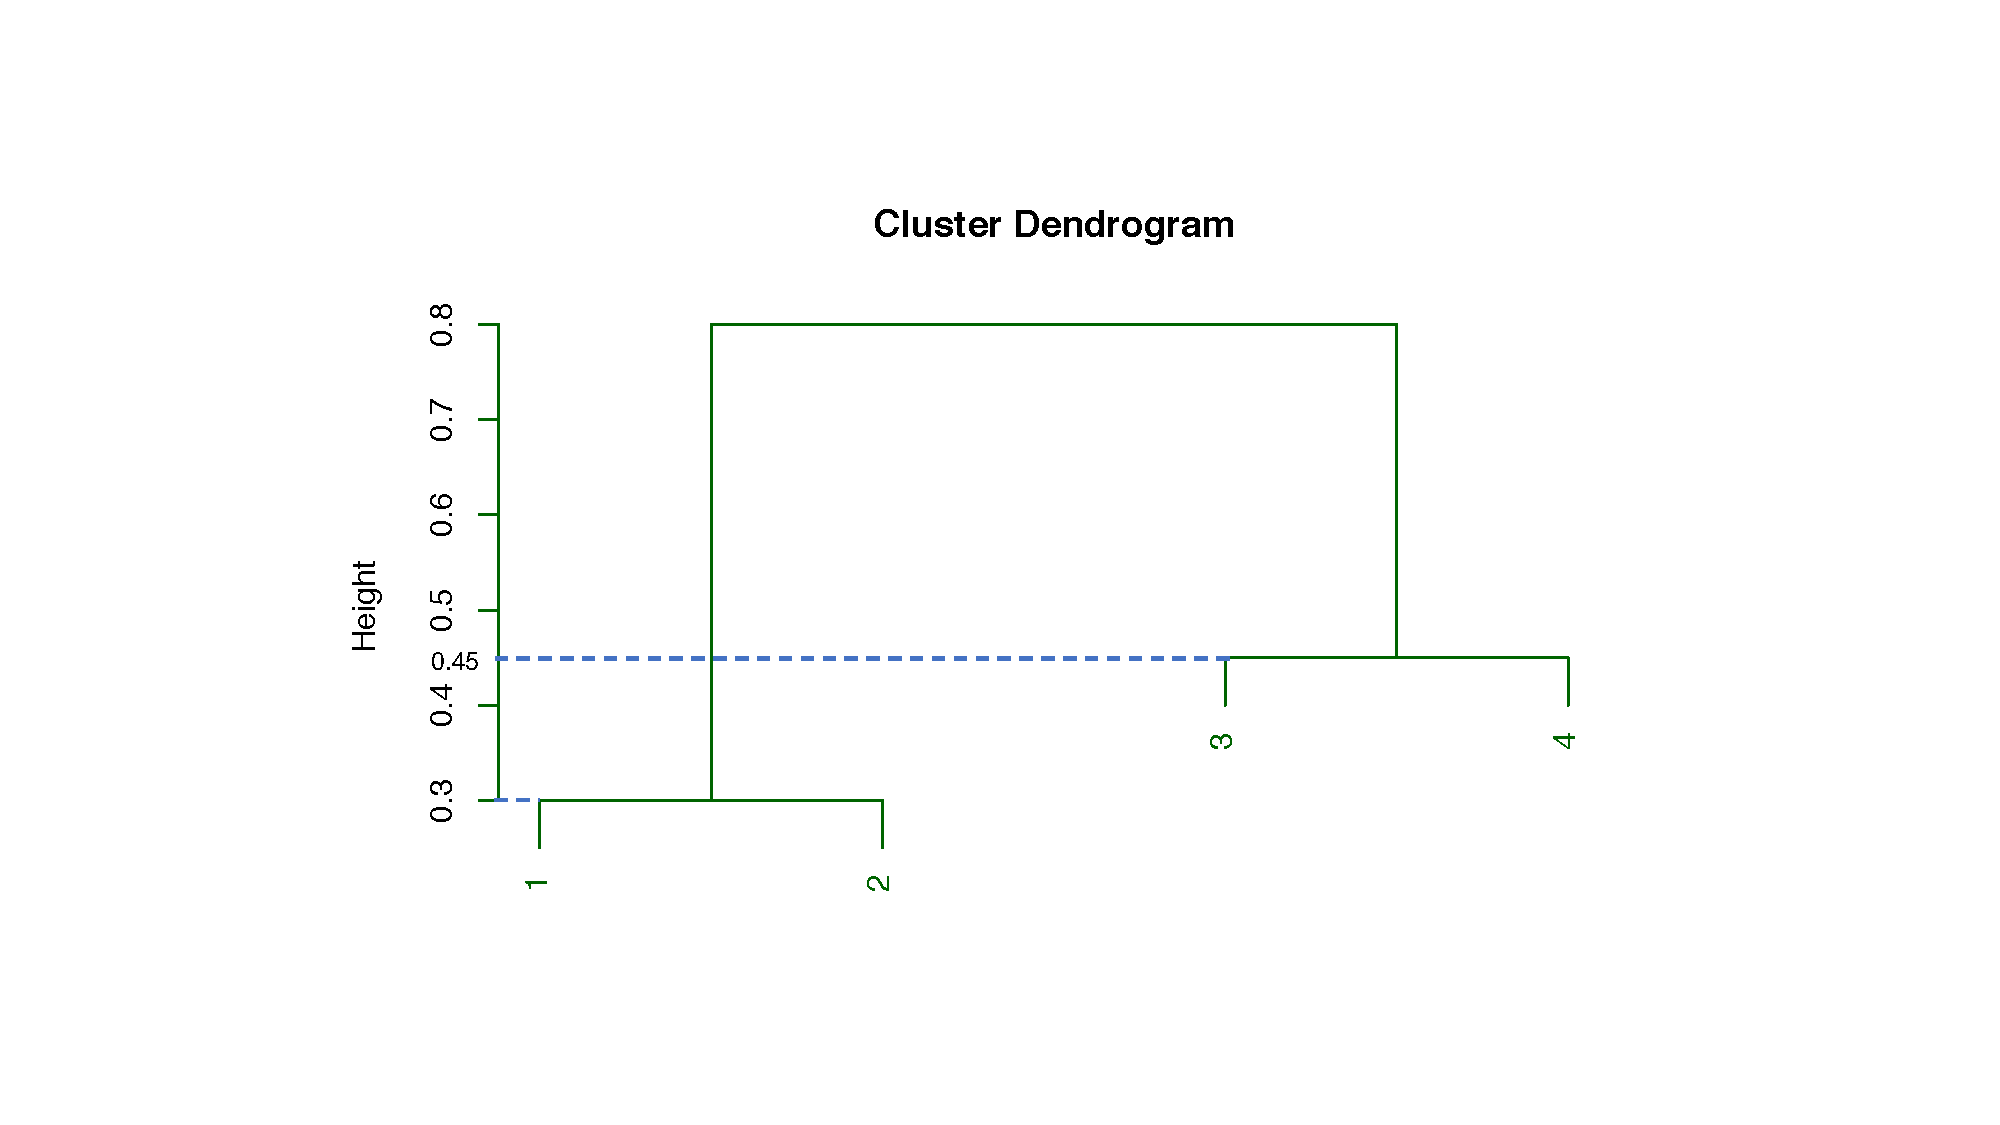
\includegraphics[width=0.75\linewidth]{Image/Prob1a.pdf}
\end{center}
\bigskip





\qnum{b}
\begin{center}
  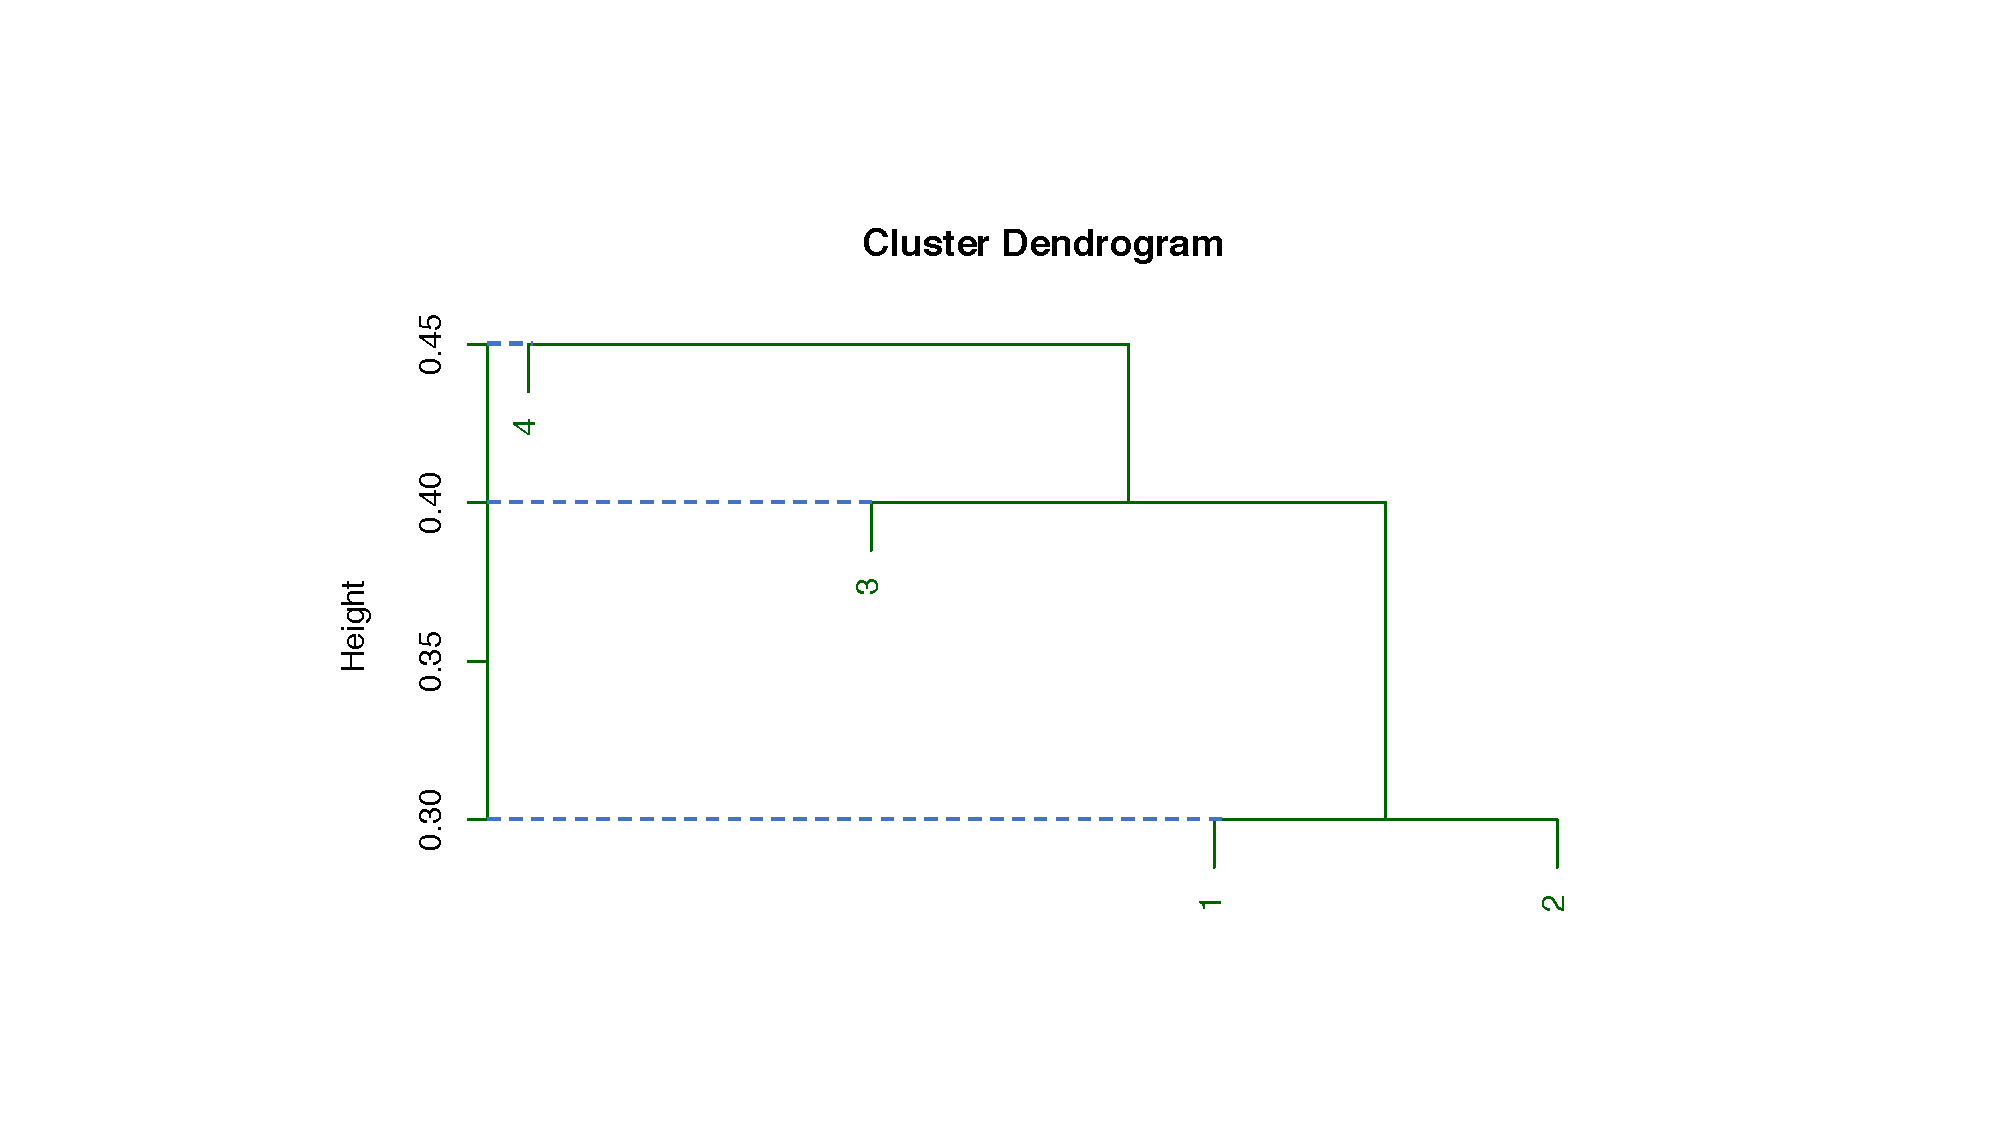
\includegraphics[width=0.75\linewidth]{Image/Prob1b.pdf}
\end{center}
\bigskip



\qnum{c}
If we cut the dendogram in (a) to obtain two clusters, say at height 0.7, then we would have the following result:
\begin{itemize}
    \item Cluster 1: Observations 1 and 2
    \item Cluster 2: Observations 3 and 4
\end{itemize}




\qnum{d}
If we cut the dendogram in (b) to obtain two clusters, then we would have the following result:
\begin{itemize}
    \item Cluster 1: Observation 4
    \item Cluster 2: Observations 1, 2 and 3
\end{itemize}


\qnum{e}
\begin{center}
  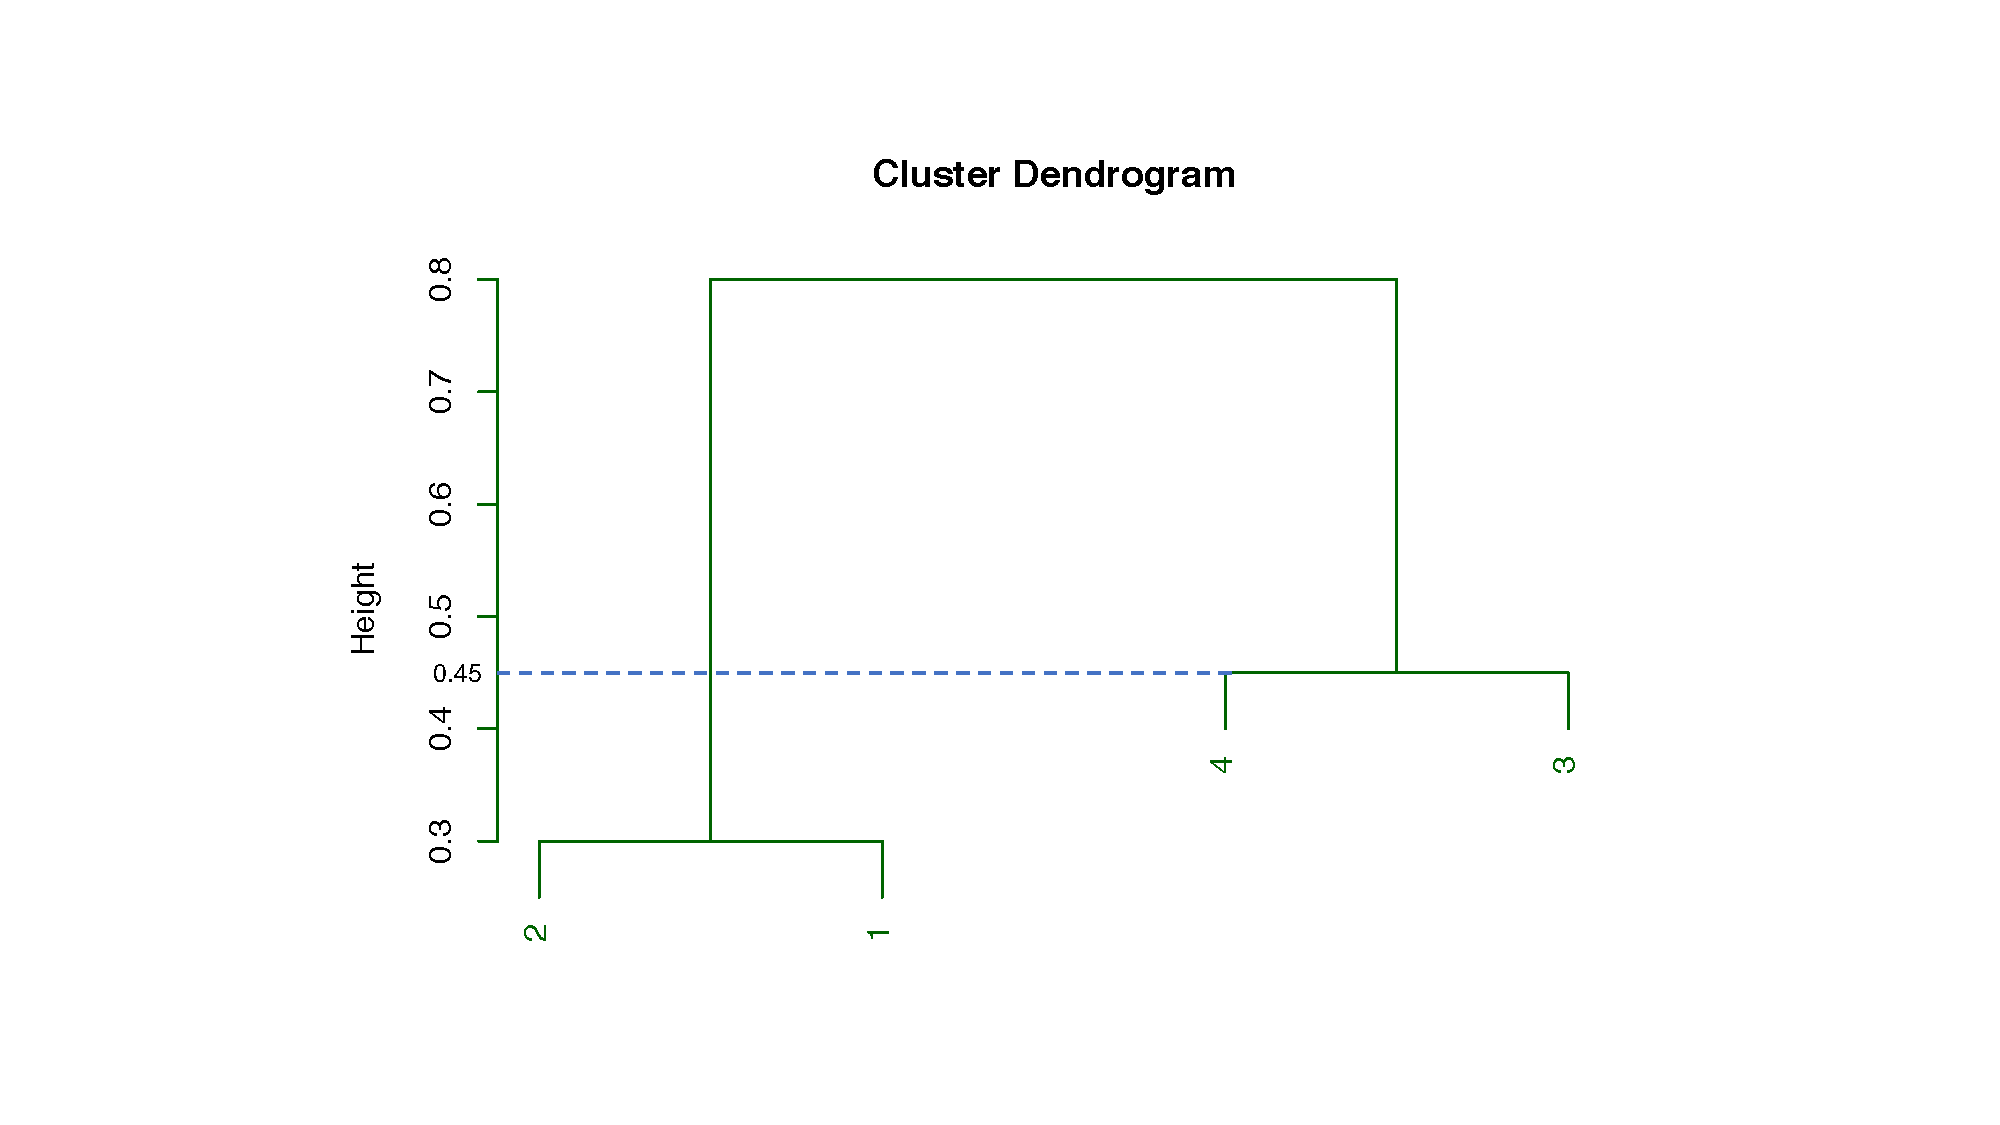
\includegraphics[width=0.75\linewidth]{Image/Prob1e.pdf}
\end{center}
\bigskip









\newpage 
 %%%%%%%%%%%%%%%%%%%%%%%%%%%%%%%%%%%%%%%%%%%%%%%%%%%%%

%     PROBLEM 2

 %%%%%%%%%%%%%%%%%%%%%%%%%%%%%%%%%%%%%%%%%%%%%%%%%%%%%


\section*{Problem 2 [50 points]} 

 Implement expectation-maximization algorithm for Gaussian mixture models (see the EM algorithm below) in \textit{R}  and call this program $G_k$. As you present your code explain your protocol for


\begin{enumerate}
  \item[3.1] initializing each Gaussian
  \item[3.2] maintaining $k$ Gaussian
  \item[3.3]  deciding ties
  \item[3.4] stopping criteria
\end{enumerate}
\sep 

\qnum{3.1}
To initialize each Gaussian, the $n$ data points are randomly labeled with \code{label 1}, \code{label 2}, $\cdots$, \code{label k}. In this way, they form $k$ different clusters. $\mu_1$, $\mu_2$, $\cdots$, $\mu_{k}\in \mathbb{R}^d$ are calculated as the center of the initial $k$ clusters, i.e.
\[
    \mu_i 
    = \frac{\displaystyle\sum_{x\text{ has \code{label i}}} x}{\text{number of $x$ with \code{label i}}},\quad 
    \text{where } x\in \Delta\subset \mathbb{R}^d, \text{ representing data point vectors}
\]
To make sure $k$ clusters are formed, after the initialization step described above, $k$ random data points are selected and labeled 1 to $k$.

All covariance matrices are initialized as the identity matrix. And all prior probabilities are initialized as $\frac{1}{k}$.
\bigskip

Another initialization method is also tested. To initialize, $\mu_1$, $\mu_2$, $\cdots$, $\mu_{k}$ are chosen to be $k$ random data points from the original observations. The covariance matrices and prior probabilities are initialized in the same way as in the previous method.
\bigskip



\qnum{3.2-3.3}
During the EM algorithm, there are no ties, as clusters are formed only at the end of the program. 

The cluster number might become less than $k$ at the end of the program when clusters are calculated according to the posterior probabilities $w_{ij}$. If this happens, then we restart the program and recluster using the algorithm, until $k$ clusters are formed.
\bigskip




\qnum{3.4}
The stopping criteria is 
\[
    \sum_{i = 1}^k \|\mu_i^t-\mu_i^{t-1}\|^2 < \code{tol}
\]
and we also cap maximum number of iterations.

The actual value for \code{tol} and maximum number of iterations are determined by experiments. Good values for those two parameters may vary with different data sets and different $k$ values. In our experiments, a maximum number of iterations of 200 and a value of tolerance $\code{tol} = 10^{-6}$ are used in the R program for the Ringnorm and Ionosphere data sets.















 %%%%%%%%%%%%%%%%%%%%%%%%%%%%%%%%%%%%%%%%%%%%%%%%%%%%%
%PROBLEM 3

 %%%%%%%%%%%%%%%%%%%%%%%%%%%%%%%%%%%%%%%%%%%%%%%%%%%%%
\newpage
\section*{Problem 3 [70 points]}

In this questions, you are asked to run your program, $G_k$, against the Ringnorm and Ionosphere data sets and compare $G_k$  with  $C_k$ ($k$-means algorithm from previous homework).  Click on the below links to download the data sets.
 \begin{itemize}
 \item  \href{http://mldata.org/repository/data/viewslug/ringnorm-ida/}{Ringnorm Data Set}
 \item  \href{https://archive.ics.uci.edu/ml/datasets/ionosphere}{
Ionosphere Data Set }
 \end{itemize}

Answer the following questions:




\begin{enumerate}
  \item[\textbf{3.1}]Initialize $G_k$ and $C_k$ with the same set of initial points (initial centroids  for $C_k$ and $\mu_i$-s for $G_k$  are identical) and run  them  for $k = 2,\ldots,5$ for 20 runs each. Report  error rates and iteration counts for each $k$ using whisker plots that reveal comparison of $C_k$ and $G_k$. An example of whisker plot is given below. A simple error rate can be calculated as follows:
  
  \begin{itemize}
  \item If $k =2$:  $C_k$ and $G_k$ will predict two clusters. Error calculation is trivial for two clusters.
  \item If $k>2$: after  $C_k$ and $G_k$ converge, combine the clusters as follows to ended up with two clusters: since the true clusters are known for a given arbitrary blocks
number, final clusters are determined by measuring the
Euclidean (this is the easiest choice) distances between
true cluster centers and predicted cluster centers.
  \end{itemize}
  
  In other words, you will always calculate the error for $k=2$ since there are only 2 clusters in the given data sets. Below is an example of error calculation for Ionosphere data set. You can  similarly calculate an error rate for Ringnorm data set.


 For each centroid $C_i$, and each Gaussian $G_k$ form two counts (over Ionosphere Data Set)  :
  \begin{eqnarray*}
  g_i &\gets& \sum_{\delta \in c_i.B} [\delta.C ==\text{\quotes{g}}],\ \ \ \mbox{\rm good}\\
  b_i &\gets& \sum_{\delta \in c_i.B} [\delta.C = =\text{\quotes{b}}], \ \ \ \mbox{\rm bad}
  \end{eqnarray*}
  where $[x = y]$ returns 1 if True, 0 otherwise.  For example, $[2 = 3] + [0 = 0] + [34 = 34] = 2$
  
  The centroid $C_i$  and Gaussian $G_k$ is classified as good if $g_i > b_i$ and bad otherwise.  We can now calculate a simple error rate.    Assume $C_i$ is good.  Then the error is:
 \begin{eqnarray*}
 error(C_i) &=& \frac{b_i}{b_i + g_i}\ \ \   \text{[same for error($G_i$)]}
 \end{eqnarray*}
 We can find the total error rate easily:
 \begin{eqnarray*}
 Error(\{C_1, C_2\}) &=& \sum_{i=1}^2 error(C_i)
 \end{eqnarray*}

  Discuss  your results, i.e., which one performs better.
  
  \item[\textbf{3.2}] In this question, we will run your $G_k$ with fixing the variances to ones and the priors to be uniform. Do not update the variances and priors throughout  iterations.  As explained in question 3.1,  compare  your new $G_k$  and $C_k$ using whisker plots. Discuss your results, i.e., which one performed better.
  
\end{enumerate}
\sep 

\qnum{3.1}
\begin{center}
    \textcolor{mydarkgreen}{\textbf{Ringnorm Data Set}}
\end{center}
\bigskip

\noindent (1) Comparison between two methods:

\begin{center}
  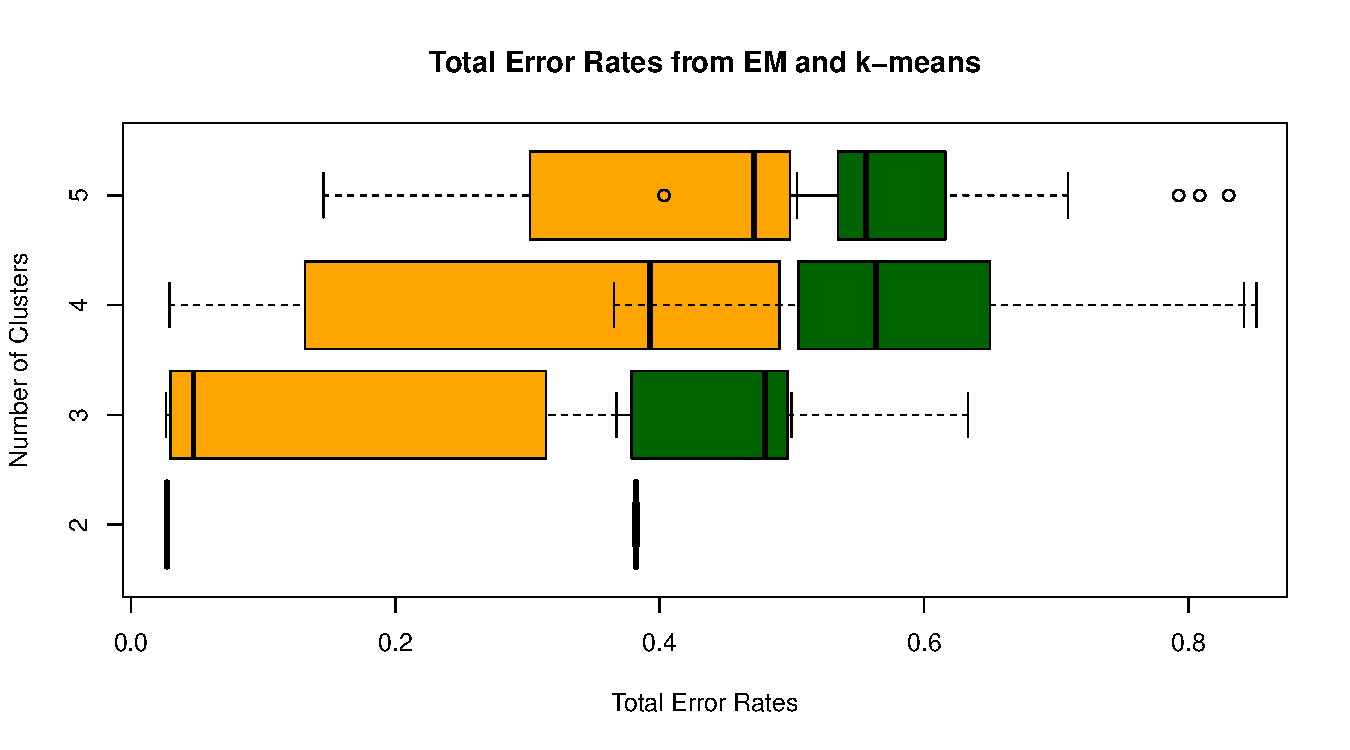
\includegraphics[width=0.9\linewidth]{Image/Prob3-TotalErr-Ringnorm-Both.pdf}
  
  % Comments
   \parbox{0.9\textwidth}{\textit{In the plot, the \textcolor{myorange}{orange boxes} represent total error rates from the EM algorithm, while the \textcolor{mydarkgreen}{green boxes} represent rates from the $k$-means algorithm.
  }}
\end{center}
\bigskip

\begin{center}
  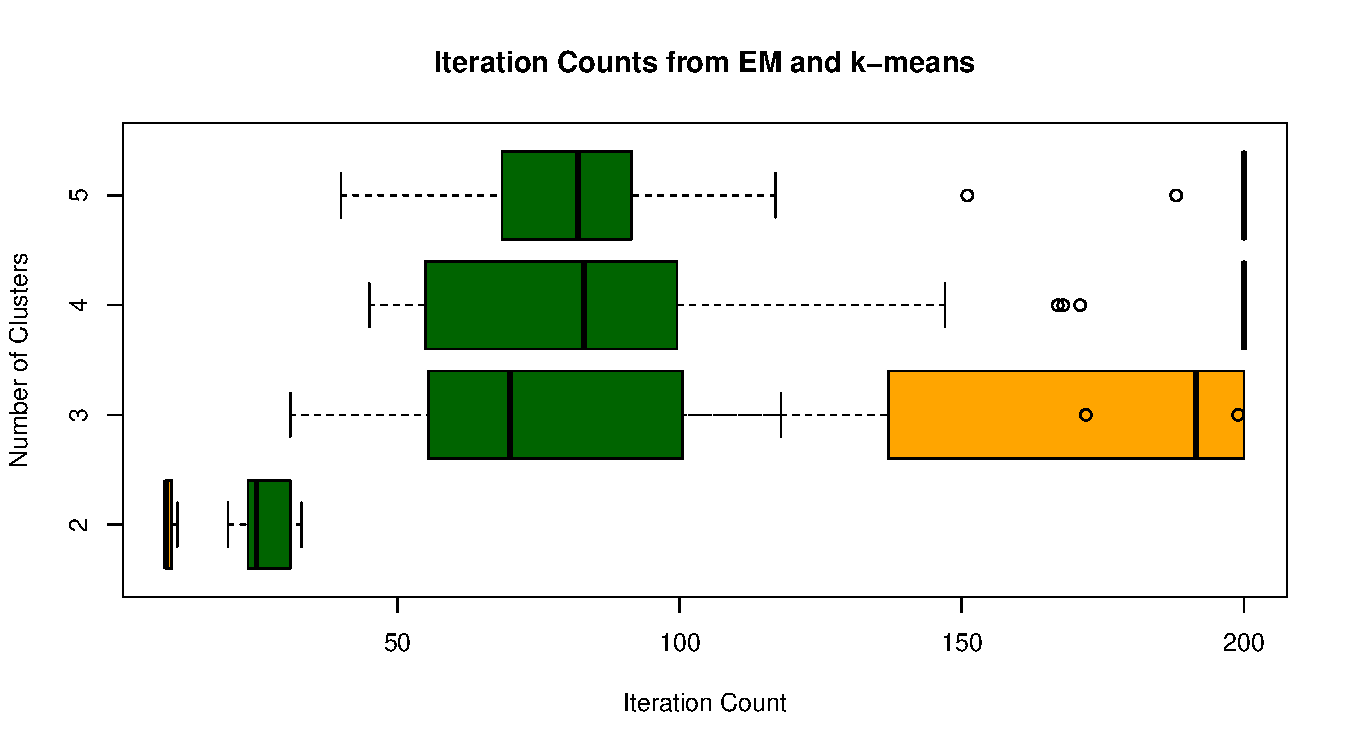
\includegraphics[width=0.9\linewidth]{Image/Prob3-ItrCount-Ringnorm-Both.pdf}
  
  % Comments
   \parbox{0.9\textwidth}{\textit{In the plot, the \textcolor{myorange}{orange boxes} represent iteration counts from the EM algorithm, while the \textcolor{mydarkgreen}{green boxes} represent counts from the $k$-means algorithm. 
   All algorithms had maximum iteration number capped at 200. The EM algorithm does not seem to converge well on $k = 4,\ 5$.
  }}
\end{center}
\bigskip

\noindent (2) EM method only:
\begin{center}
  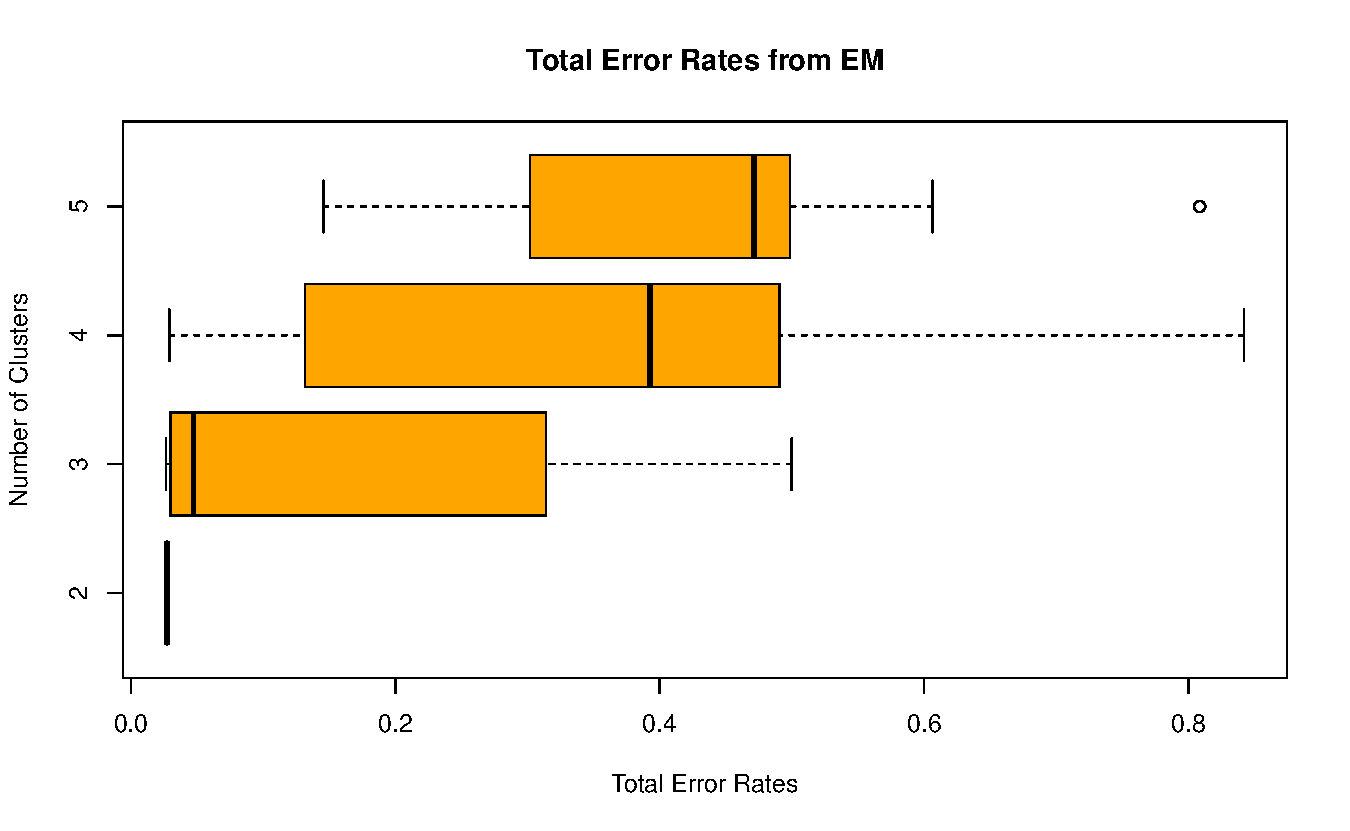
\includegraphics[width=0.8\linewidth]{Image/Prob3-TotalErr-Ringnorm-EM.pdf}
\end{center}
\begin{center}
  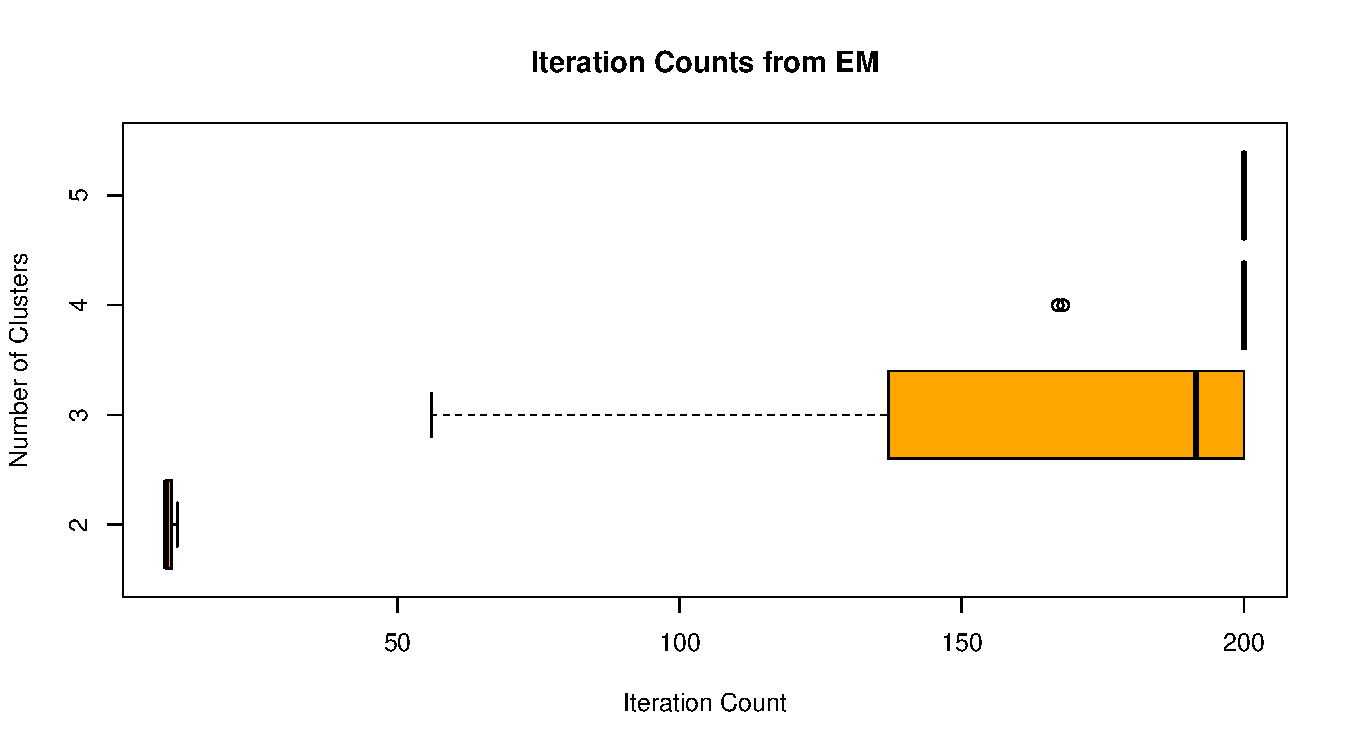
\includegraphics[width=0.8\linewidth]{Image/Prob3-ItrCount-Ringnorm-EM.pdf}
\end{center}
\bigskip

\noindent (3) $k$-means method only:
\begin{center}
  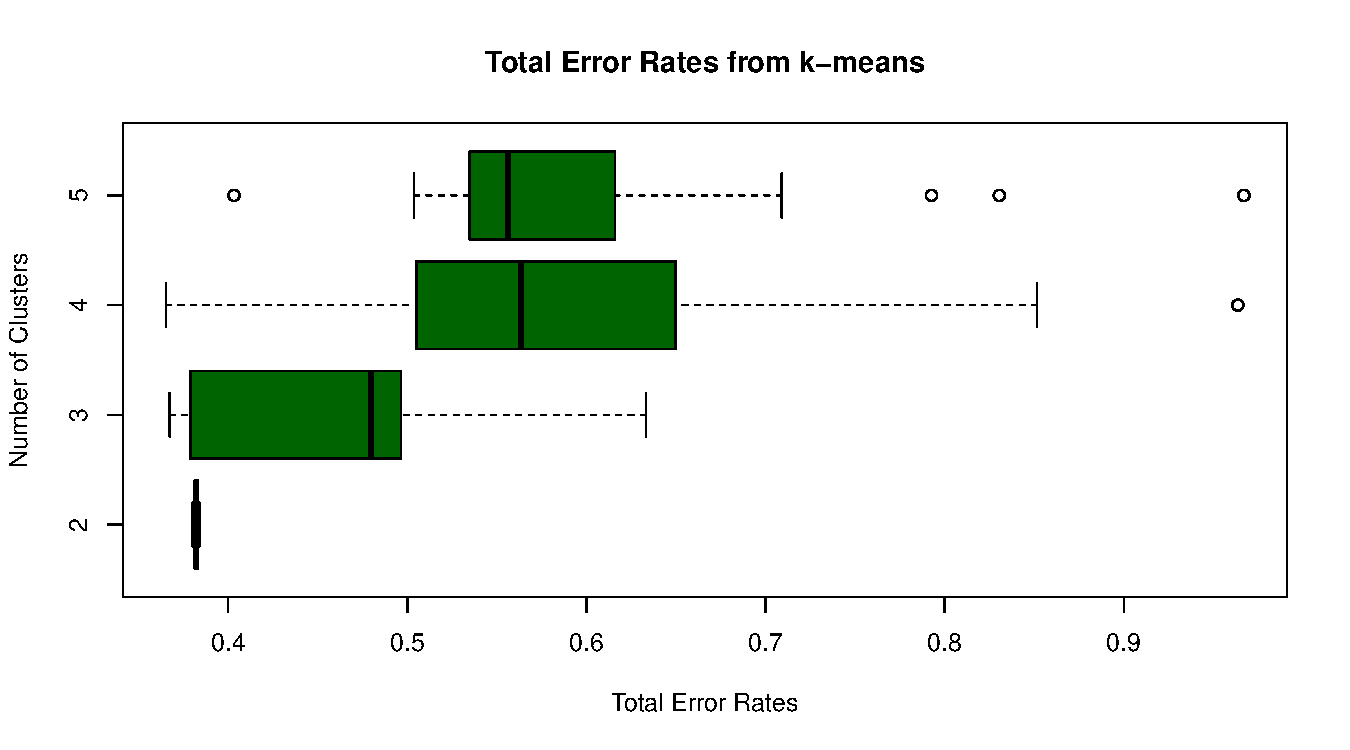
\includegraphics[width=0.8\linewidth]{Image/Prob3-TotalErr-Ringnorm-kmeans.pdf}
\end{center}
\begin{center}
  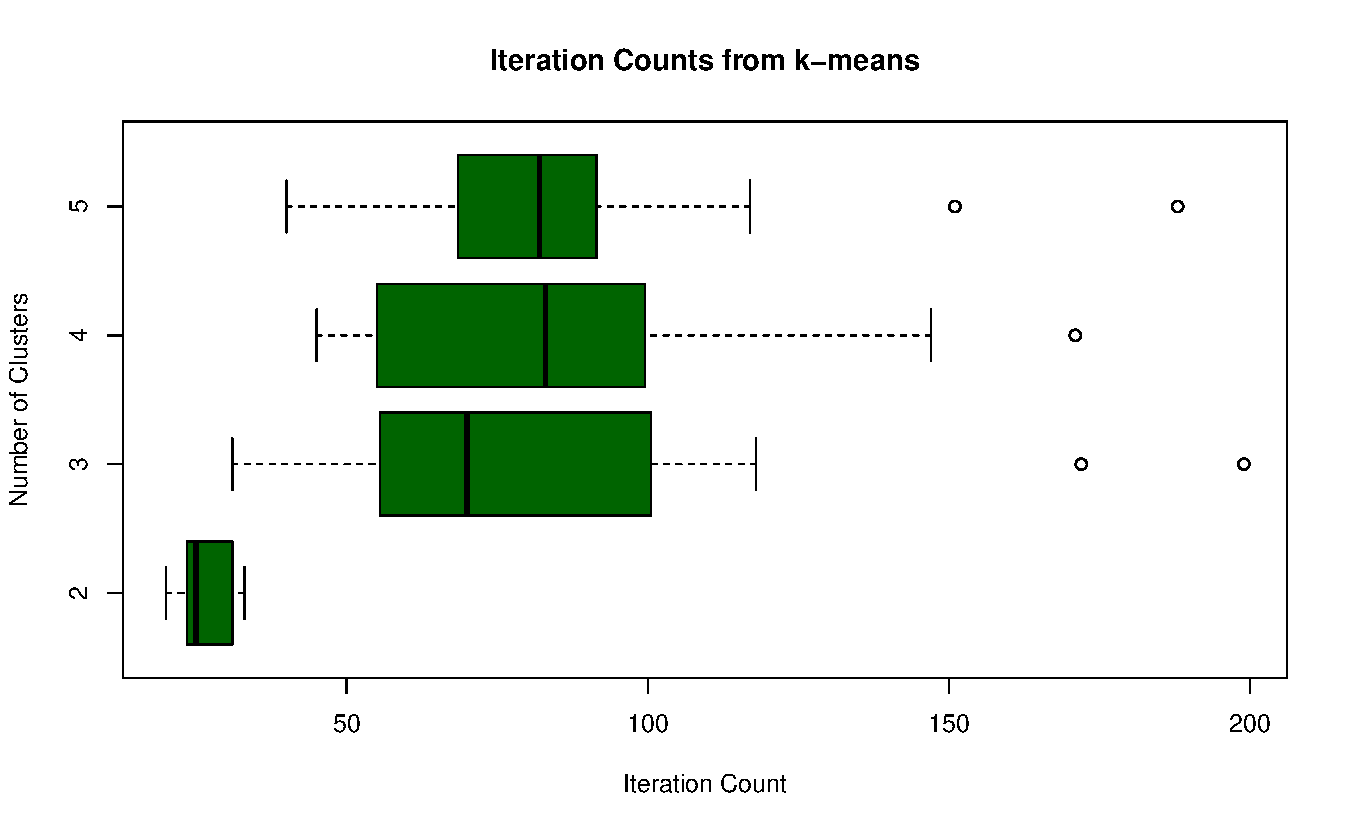
\includegraphics[width=0.8\linewidth]{Image/Prob3-ItrCount-Ringnorm-kmeans.pdf}
\end{center}







\bigskip
\begin{center}
    \textcolor{mydarkgreen}{\textbf{Ionosphere Data Set}}
\end{center}

\noindent (1) Comparison between two methods:

\begin{center}
  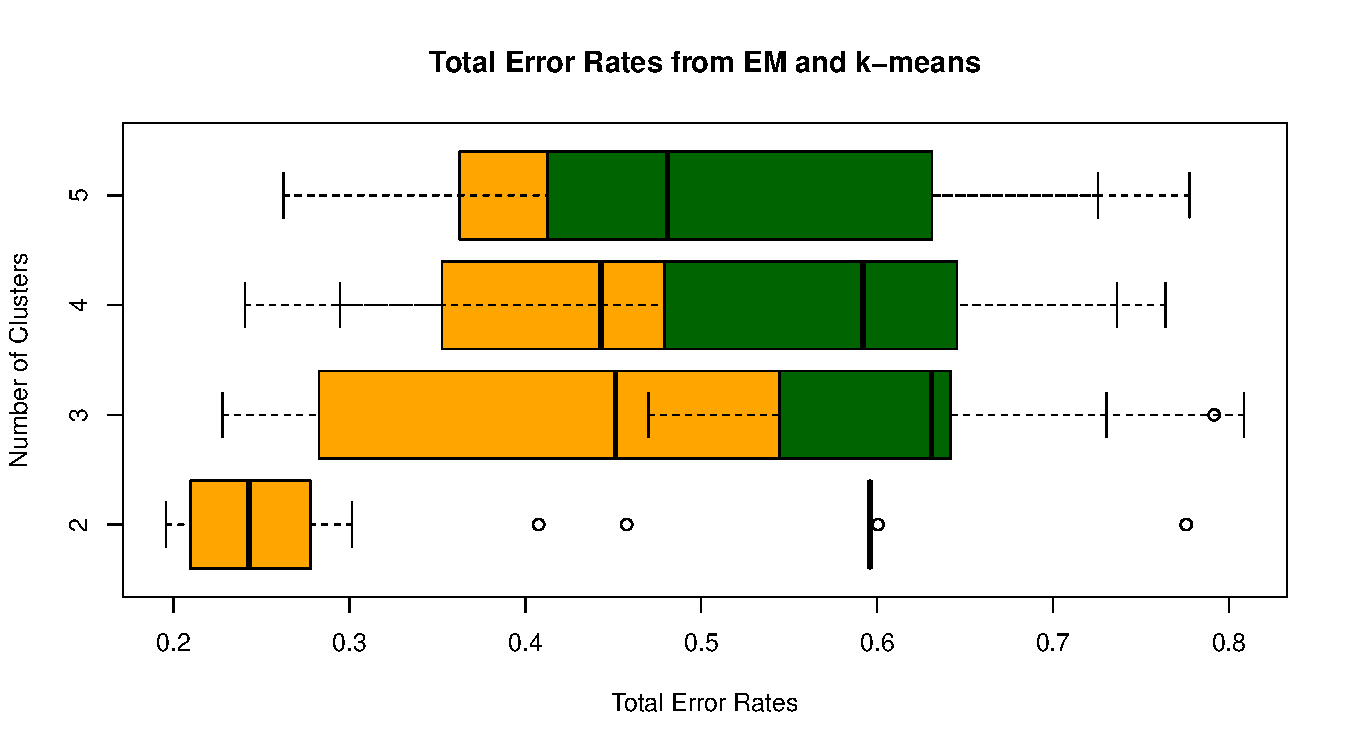
\includegraphics[width=0.9\linewidth]{Image/Prob3-TotalErr-Ionosphere-Both.pdf}
  
  % Comments
   \parbox{0.9\textwidth}{\textit{In the plot, the \textcolor{myorange}{orange boxes} represent total error rates from the EM algorithm, while the \textcolor{mydarkgreen}{green boxes} represent rates from the $k$-means algorithm.
  }}
\end{center}
\bigskip

\begin{center}
  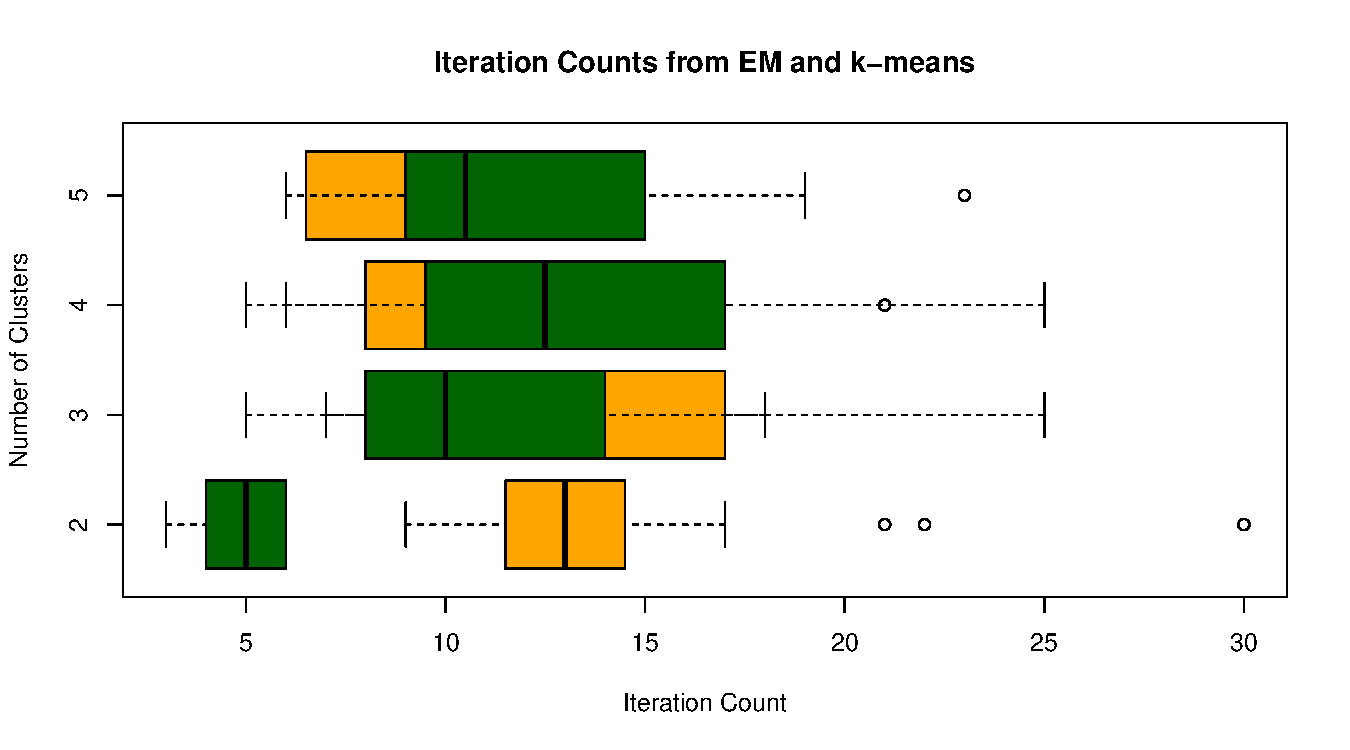
\includegraphics[width=0.9\linewidth]{Image/Prob3-ItrCount-Ionosphere-Both.pdf}
  
  % Comments
   \parbox{0.9\textwidth}{\textit{In the plot, the \textcolor{myorange}{orange boxes} represent iteration counts from the EM algorithm, while the \textcolor{mydarkgreen}{green boxes} represent counts from the $k$-means algorithm. 
   All algorithms had maximum iteration number capped at 200. 
  }}
\end{center}
\bigskip

\noindent (2) EM method only:
\begin{center}
  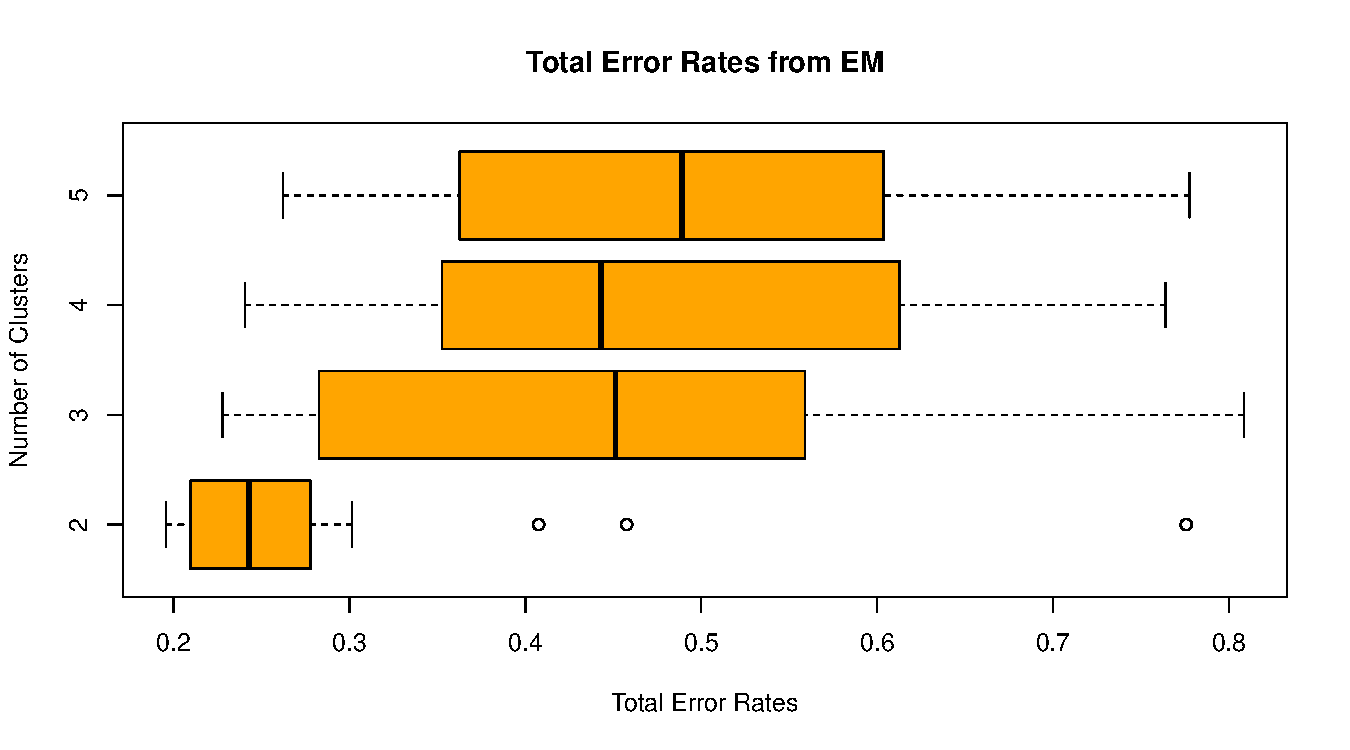
\includegraphics[width=0.8\linewidth]{Image/Prob3-TotalErr-Ionosphere-EM.pdf}
\end{center}
\begin{center}
  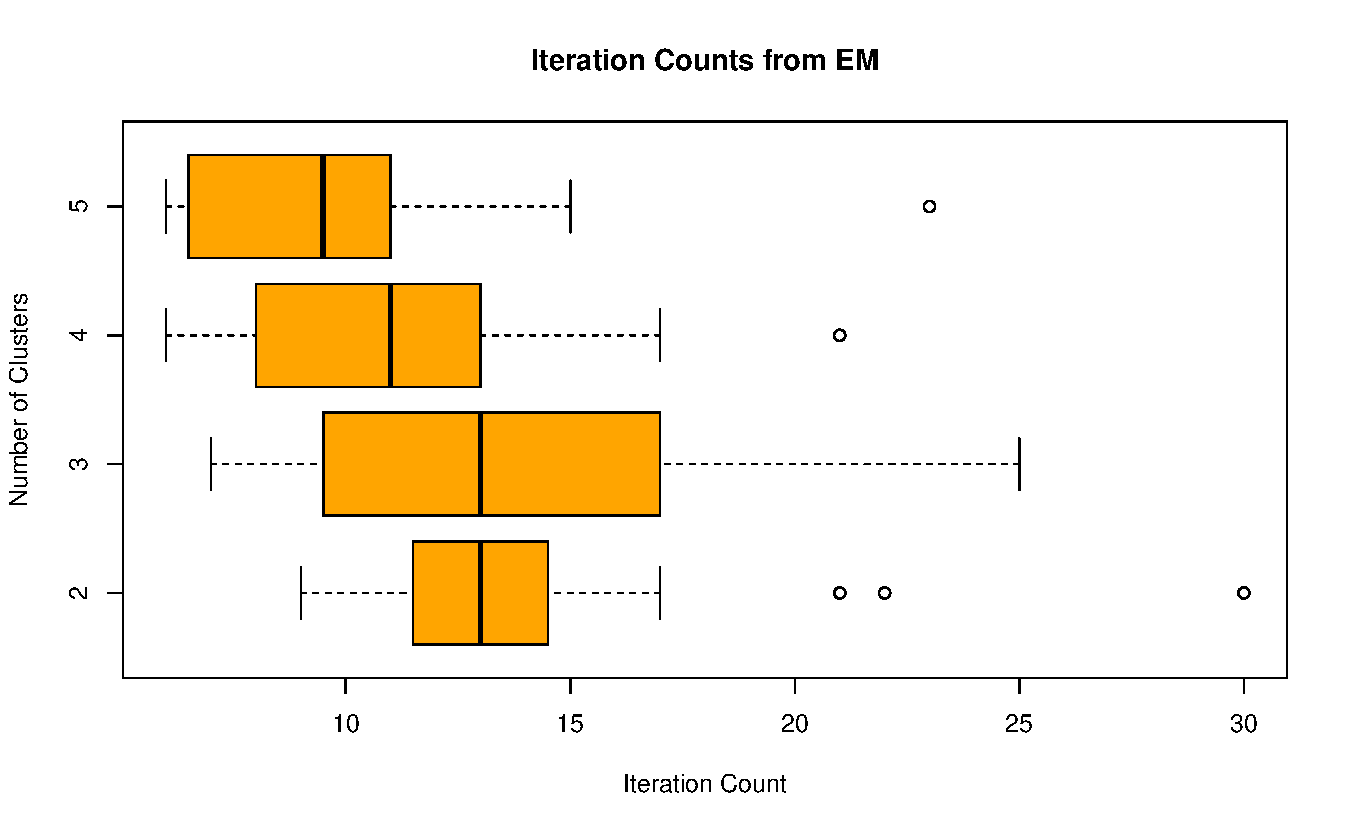
\includegraphics[width=0.8\linewidth]{Image/Prob3-ItrCount-Ionosphere-EM.pdf}
\end{center}
\bigskip

\noindent (3) $k$-means method only:
\begin{center}
  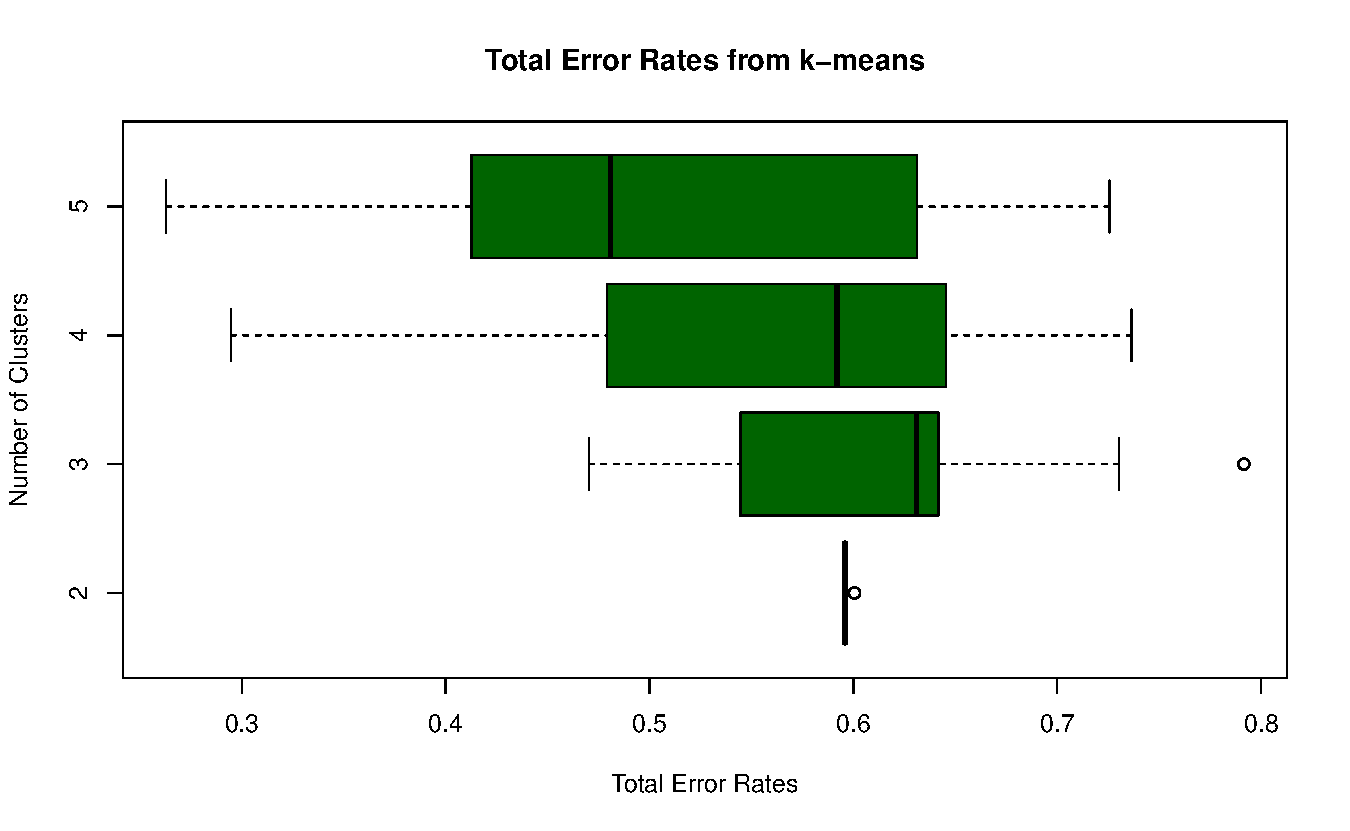
\includegraphics[width=0.8\linewidth]{Image/Prob3-TotalErr-Ionosphere-kmeans.pdf}
\end{center}
\begin{center}
  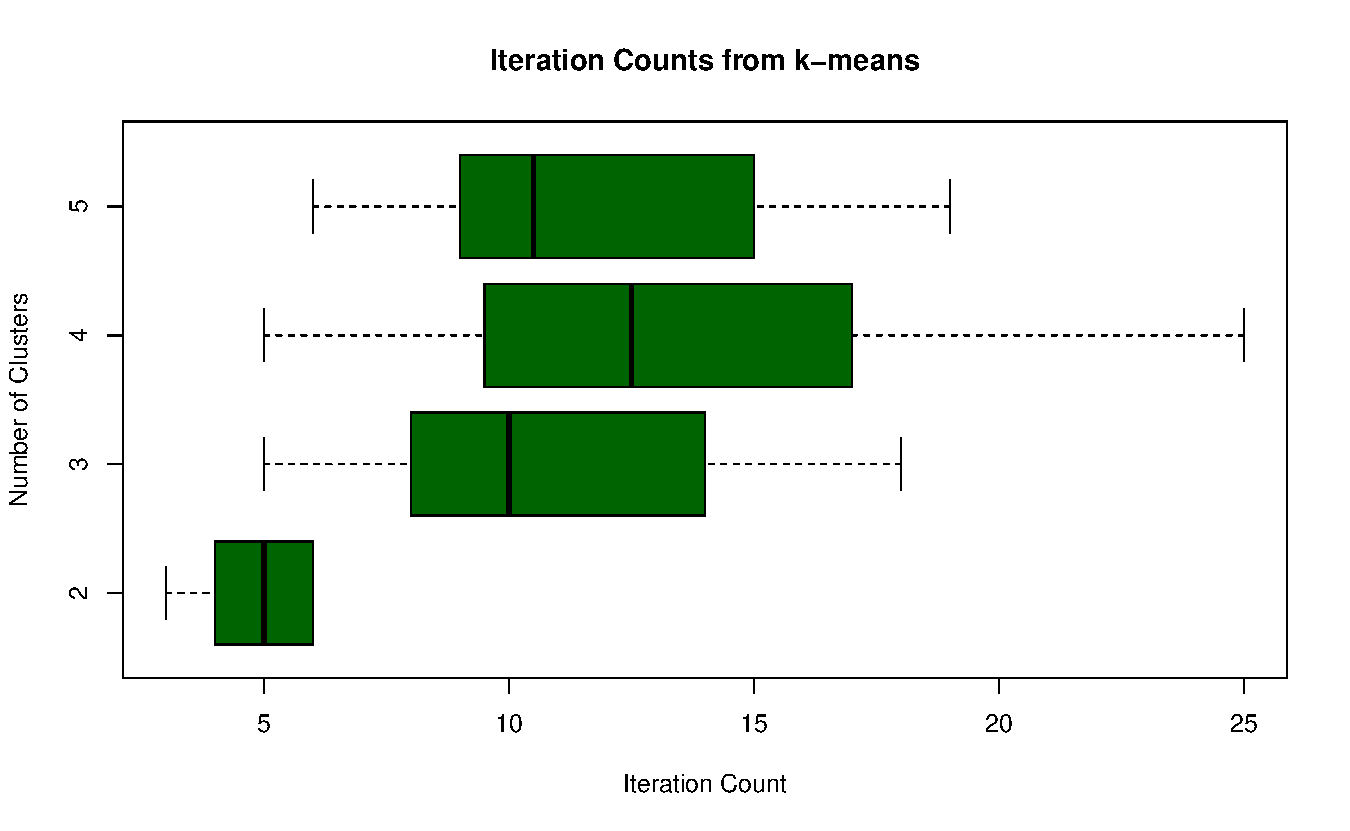
\includegraphics[width=0.8\linewidth]{Image/Prob3-ItrCount-Ionosphere-kmeans.pdf}
\end{center}




\bigskip
\begin{center}
    \textcolor{mydarkgreen}{\textbf{Analysis of Results}}
\end{center}

\noindent 
(1) \emph{On the Ringnorm data set.}

In this data set, the EM performs significantly better on the total error rates for all $k$.

On the iteration counts, the EM algorithm works better than $k$-means when $k=2$. For $k=3,\ 4,$ and 5, the EM algorithm does not converge well. But when capped at a maximum of 200 iterations, the EM already reaches better error rates than the $k$-means.

One thing to note about the comparison of iteration counts is that, for \emph{my} implementations of the EM and $k$-means algorithms in R, this comparison does not reflect the comparison of actual run time of the two algorithms. In \emph{my} implementations, EM is much more efficient than the \km algorithm, partly due to the efficiency of matrix computations in \code{R}. In a typical run, the EM takes around 6 min for all $4\times 20$ runs, whereas the \km runs around 70 min. This might change if the implementation changes, e.g. if the code is written in \code{C} instead. In our experiment, there is no conclusion on the runtime performance of the algorithms. We can only compare the performances on our \code{R} implementations.
\bigskip\bigskip


\noindent 
(2) \emph{On the Ionosphere data set.}

In this data set, the EM performs better on the total error rates in general. EM gives significantly lower total error rates for $k=2$. For other $k$ values, however, the EM gives better error rates but the difference from \km is less significant.

On the iteration counts, the EM algorithm uses more iterations than $k$-means when $k=2$. For $k=3,\ 4,$ and 5, the two algorithms use comparable number of iterations.

The issue on the comparison of actual run time mentioned in the last paragraph of (1) also applies here.
\bigskip\bigskip




\qnum{2}
\begin{center}
    \textcolor{mydarkgreen}{\textbf{Ringnorm Data Set With Second Version of EM}}
\end{center}
\vspace{10pt}

\noindent (1) Comparison between two methods:

\begin{center}
  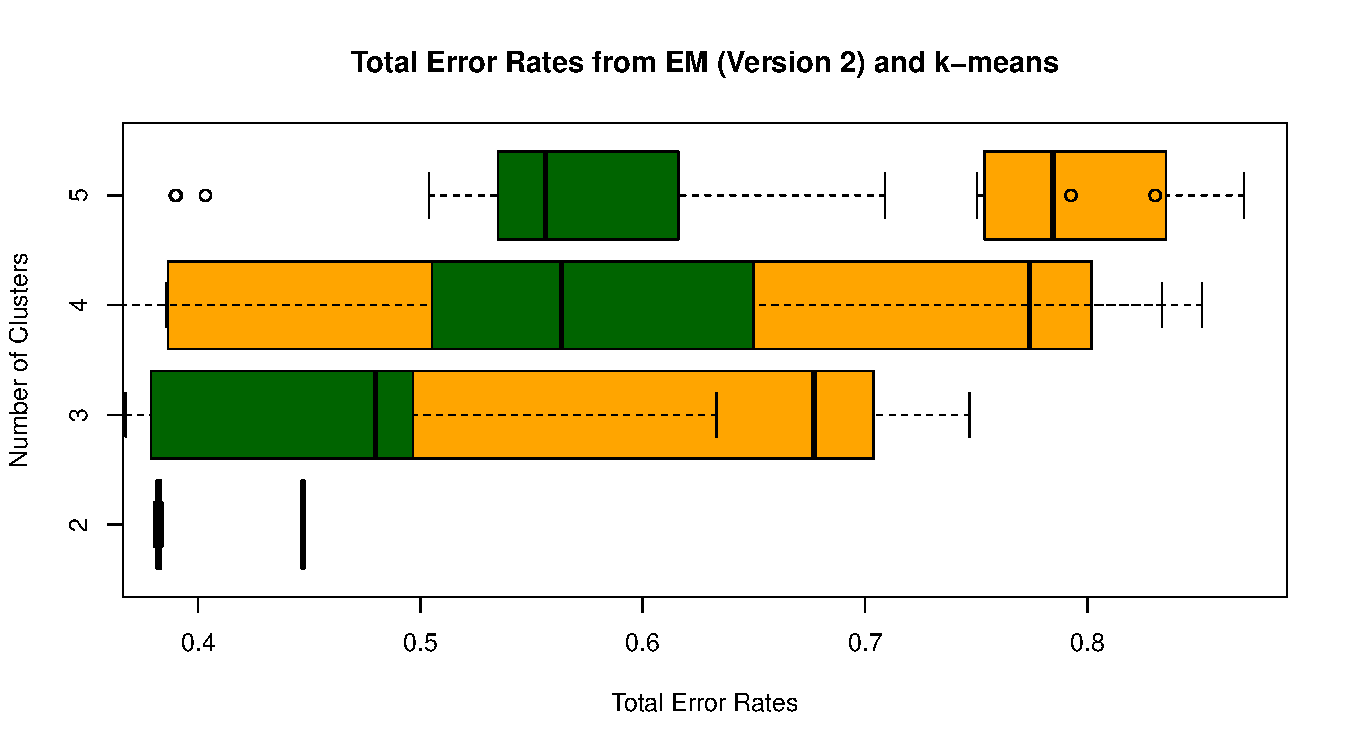
\includegraphics[width=0.9\linewidth]{Image/Prob3-2-TotalErr-Ringnorm-Both.pdf}
  
  % Comments
   \parbox{0.9\textwidth}{\textit{In the plot, the \textcolor{myorange}{orange boxes} represent total error rates from the EM algorithm, while the \textcolor{mydarkgreen}{green boxes} represent rates from the $k$-means algorithm.
  }}
\end{center}
\bigskip

\begin{center}
  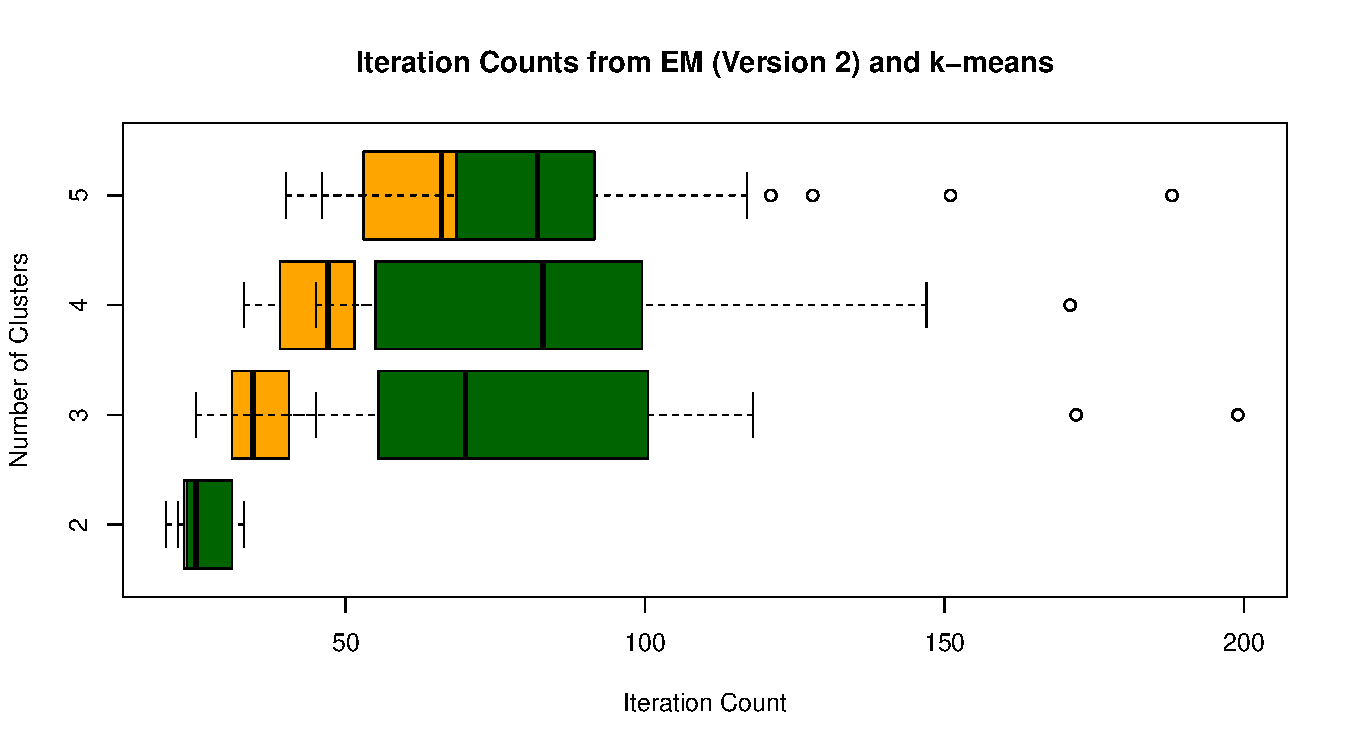
\includegraphics[width=0.9\linewidth]{Image/Prob3-2-ItrCount-Ringnorm-Both.pdf}
  
  % Comments
   \parbox{0.9\textwidth}{\textit{In the plot, the \textcolor{myorange}{orange boxes} represent iteration counts from the EM algorithm, while the \textcolor{mydarkgreen}{green boxes} represent counts from the $k$-means algorithm. 
   All algorithms had maximum iteration number capped at 200. The EM algorithm does not seem to converge well on $k = 4,\ 5$.
  }}
\end{center}
\bigskip

\noindent (2) EM method only:
\begin{center}
  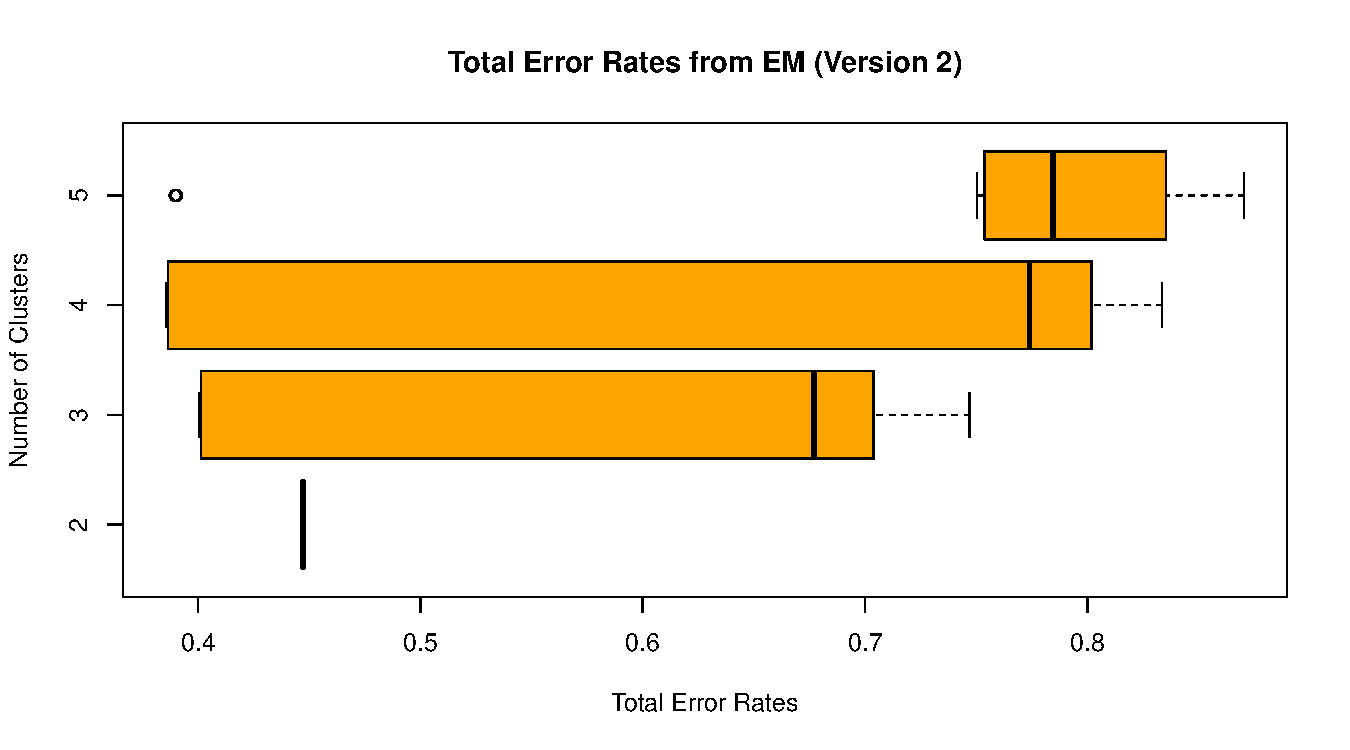
\includegraphics[width=0.8\linewidth]{Image/Prob3-2-TotalErr-Ringnorm-EMFixed.pdf}
\end{center}
\begin{center}
  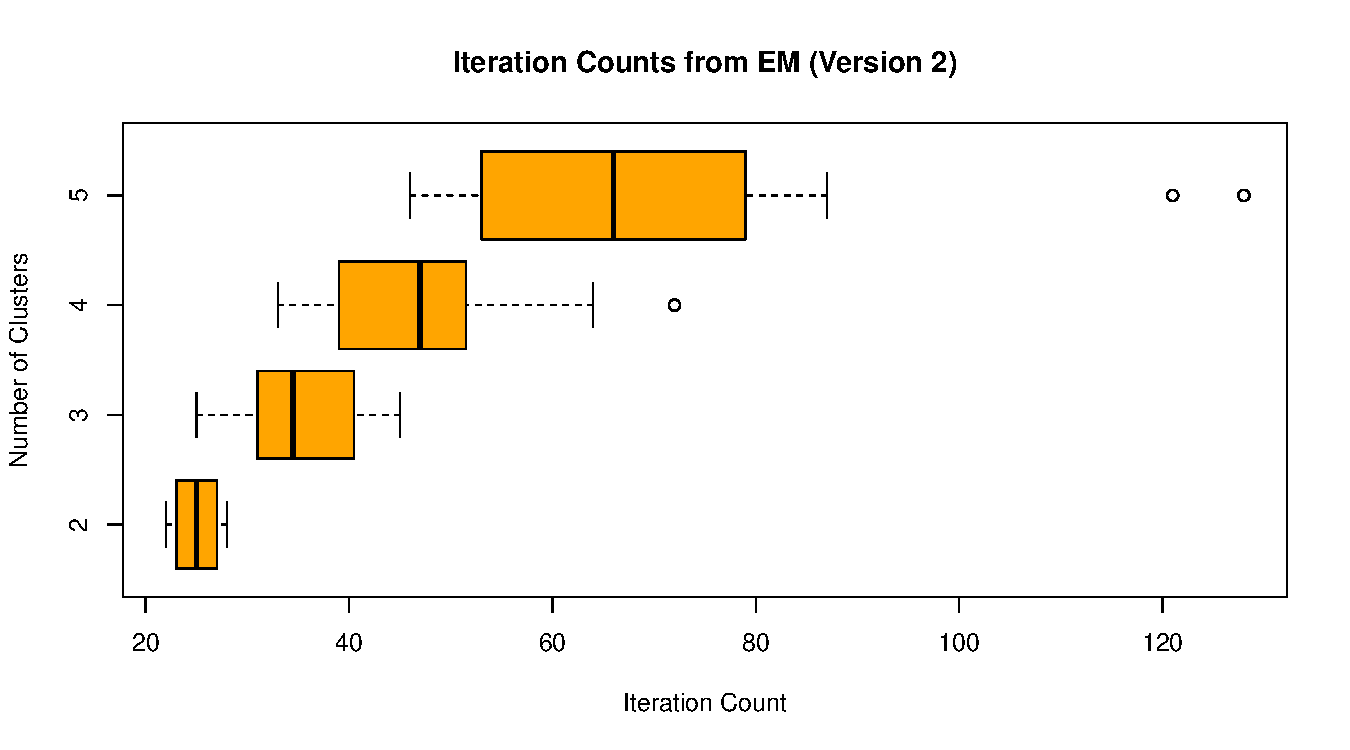
\includegraphics[width=0.8\linewidth]{Image/Prob3-2-ItrCount-Ringnorm-EMFixed.pdf}
\end{center}
\bigskip

\noindent (3) $k$-means method only:
\begin{center}
  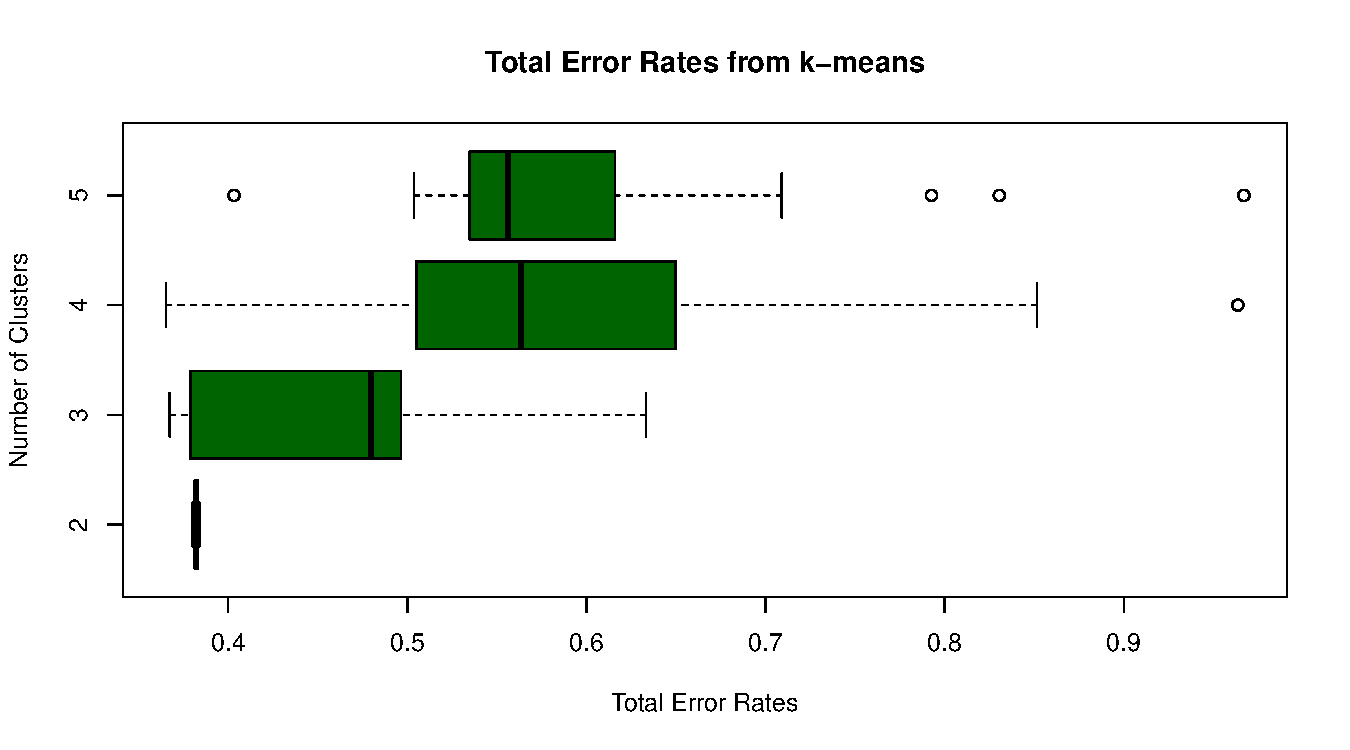
\includegraphics[width=0.8\linewidth]{Image/Prob3-TotalErr-Ringnorm-kmeans.pdf}
\end{center}
\begin{center}
  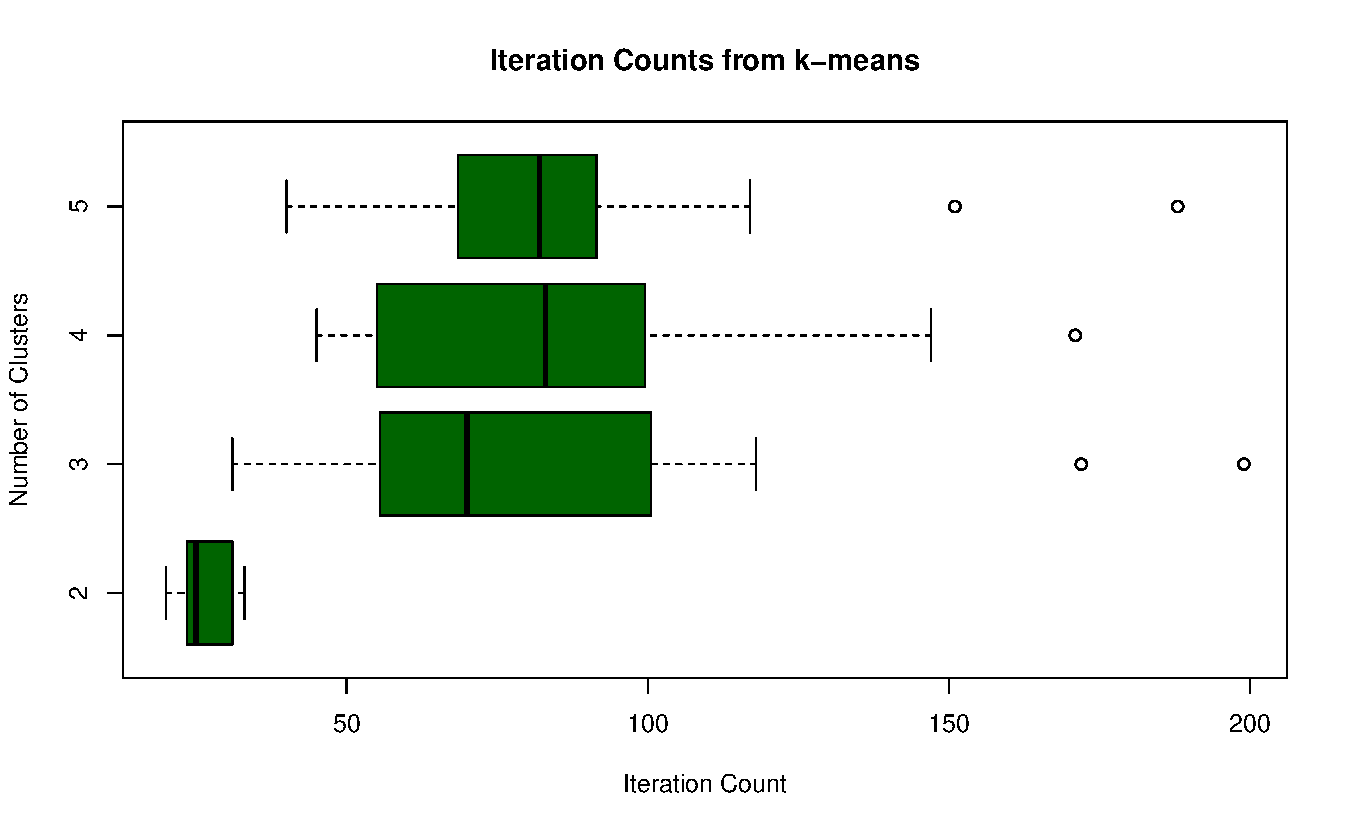
\includegraphics[width=0.8\linewidth]{Image/Prob3-ItrCount-Ringnorm-kmeans.pdf}
\end{center}










\bigskip
\begin{center}
    \textcolor{mydarkgreen}{\textbf{Ionosphere Data Set With Second Version EM}}
\end{center}

\noindent (1) Comparison between two methods:

\begin{center}
  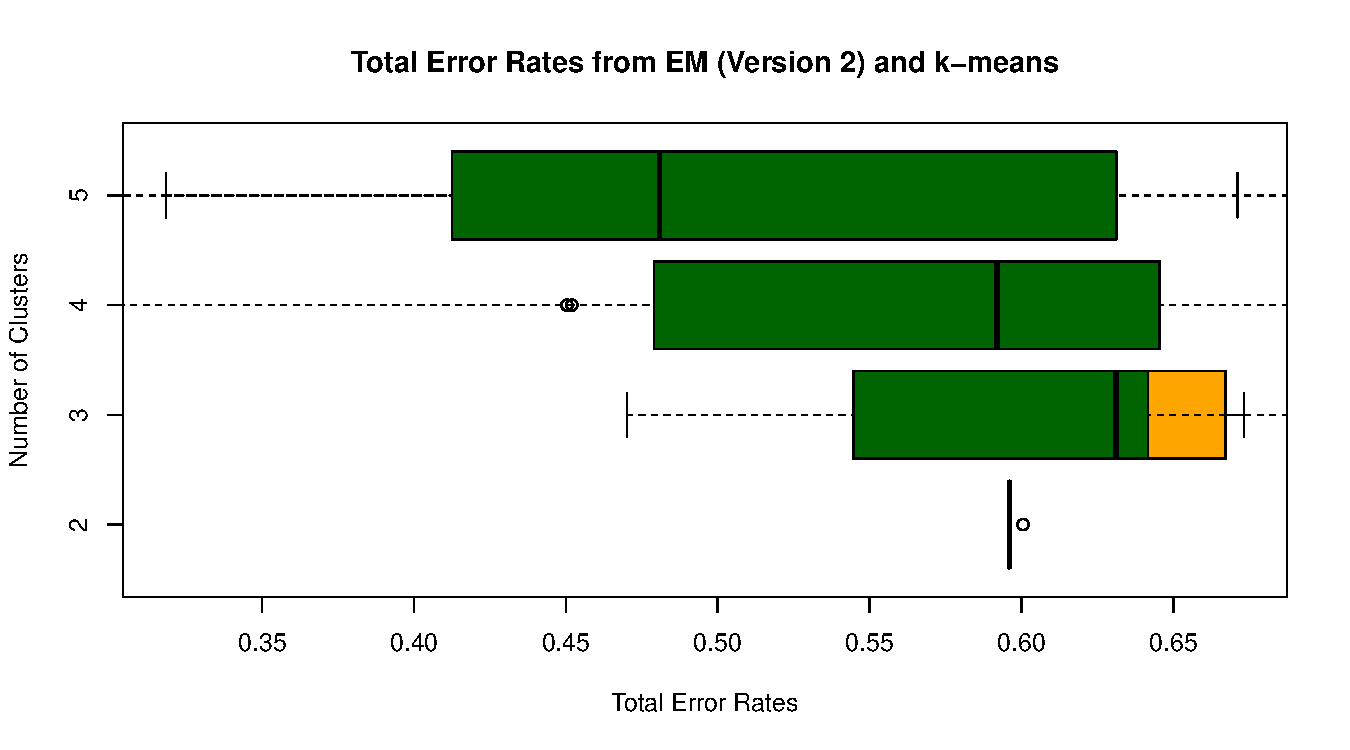
\includegraphics[width=0.9\linewidth]{Image/Prob3-2-TotalErr-Ionosphere-Both.pdf}
  
  % Comments
   \parbox{0.9\textwidth}{\textit{In the plot, the \textcolor{myorange}{orange boxes} represent total error rates from the EM algorithm, while the \textcolor{mydarkgreen}{green boxes} represent rates from the $k$-means algorithm.
  }}
\end{center}
\bigskip

\begin{center}
  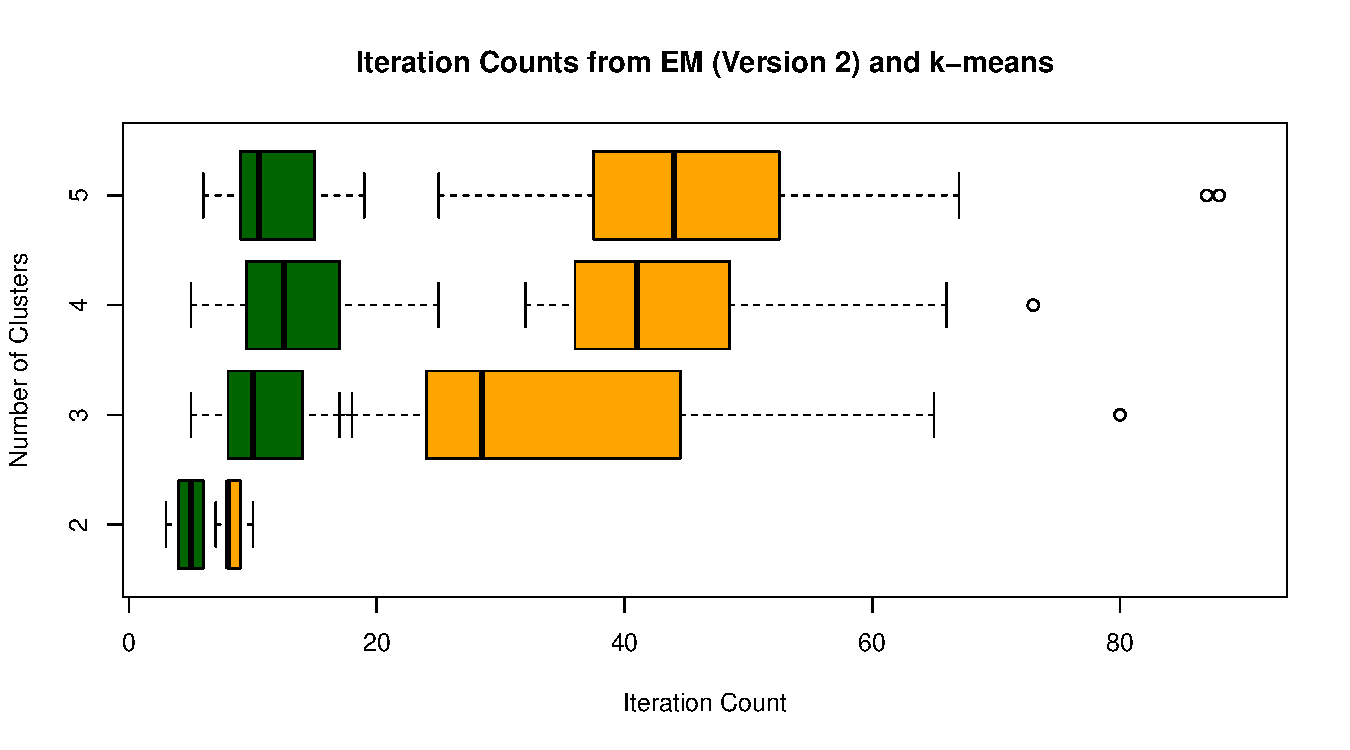
\includegraphics[width=0.9\linewidth]{Image/Prob3-2-ItrCount-Ionosphere-Both.pdf}
  
  % Comments
   \parbox{0.9\textwidth}{\textit{In the plot, the \textcolor{myorange}{orange boxes} represent iteration counts from the EM algorithm, while the \textcolor{mydarkgreen}{green boxes} represent counts from the $k$-means algorithm. 
  }}
\end{center}
\bigskip

\noindent (2) EM method only:
\begin{center}
  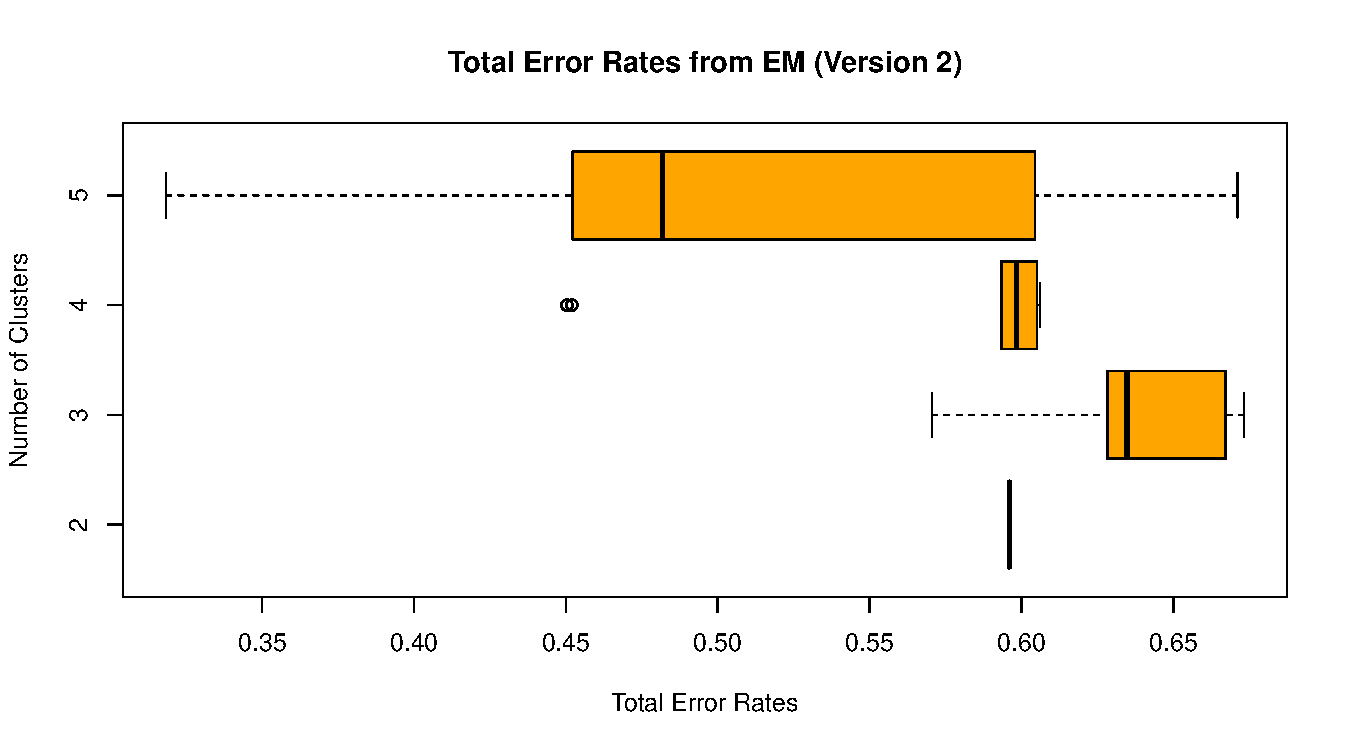
\includegraphics[width=0.8\linewidth]{Image/Prob3-2-TotalErr-Ionosphere-EMFixed.pdf}
\end{center}
\begin{center}
  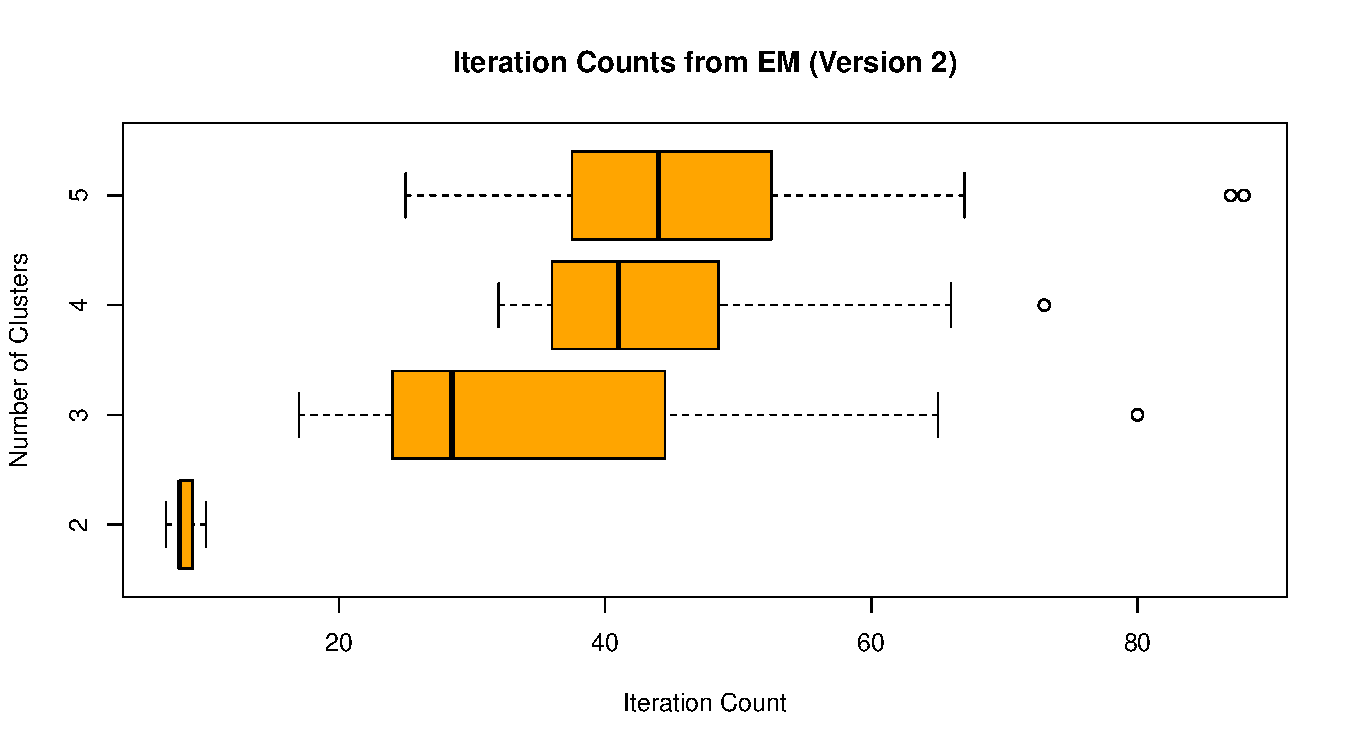
\includegraphics[width=0.8\linewidth]{Image/Prob3-2-ItrCount-Ionosphere-EMFixed.pdf}
\end{center}
\bigskip

\noindent (3) $k$-means method only:
\begin{center}
  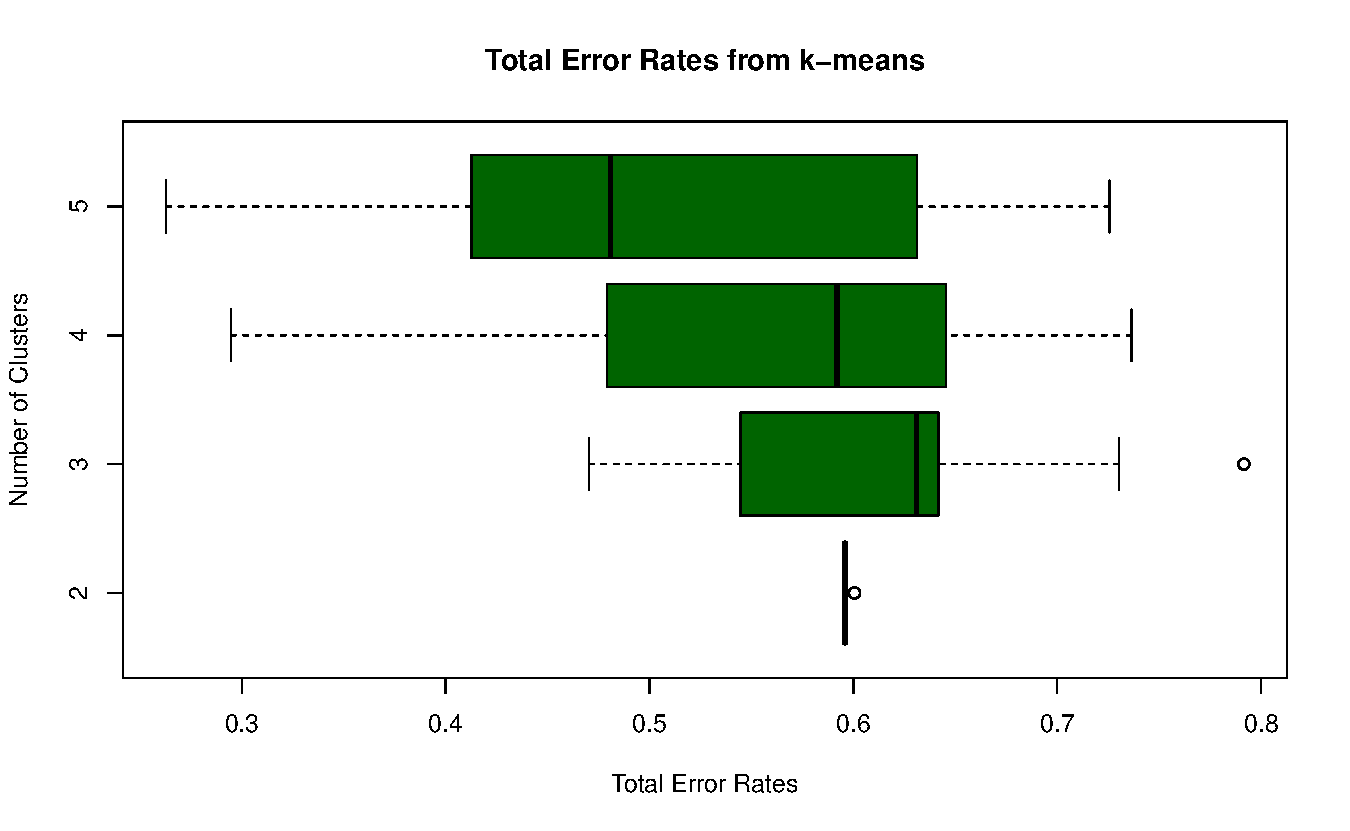
\includegraphics[width=0.8\linewidth]{Image/Prob3-TotalErr-Ionosphere-kmeans.pdf}
\end{center}
\begin{center}
  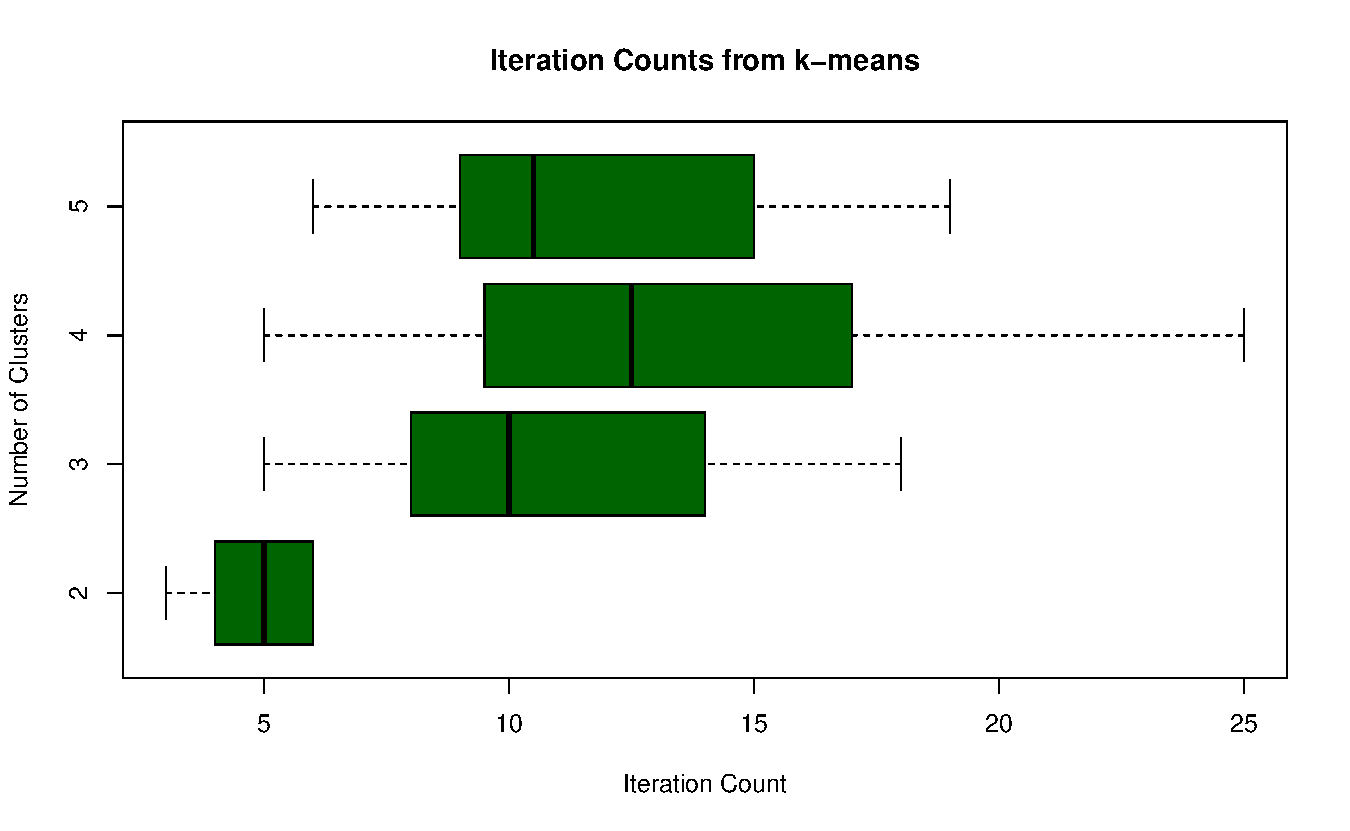
\includegraphics[width=0.8\linewidth]{Image/Prob3-ItrCount-Ionosphere-kmeans.pdf}
\end{center}





\bigskip
\begin{center}
    \textcolor{mydarkgreen}{\textbf{Analysis of Results}}
\end{center}

\noindent 
(1) \emph{On the Ringnorm data set.}

In this data set, the EM algorithm with fixed prior probabilities and covariances performs worse than $k$-means on the total error rates.
The difference is significant for $k=2$ and 5. And the variances of the errors is significantly larger than those from \km for $k=3$ and 4.



On the iteration counts, however, this version of EM uses fewer iterations than \km to converge (for all $k$). 
\bigskip\bigskip


\noindent 
(2) \emph{On the Ionosphere data set.}

In this data set, the EM (2nd version) has very similar performance as $k$-means on the total error rates.

On the iteration counts, the EM algorithm uses significantly more iterations to converge than $k$-means. 
\bigskip\bigskip


















 
 %%%%%%%%%%%%%%%%%%%%%%%%%%%%%%%%%%%%%%%%%%%%%%%%%%%%%
 

  %%%%%%%%%%%%%%%%%%%%%%%%%%%%%%%%%%%%%%%%%%%%%%%%%%%%%
%PROBLEM 4

 %%%%%%%%%%%%%%%%%%%%%%%%%%%%%%%%%%%%%%%%%%%%%%%%%%%%%

\newpage 
\section*{Problem 4 [50 points]}  
  
In this question, you will first perform principal component analysis (PCA) over Ionosphere and Rignorm data sets and then cluster the  reduced data sets using $G_k$ (from question 3.1) and $C_k$. You are allowed to use R packages for PCA.
Ignore the class variables (35th and 1st variables for Ionosphere  and Ringnorm data sets, respectively) while performing PCA. Answer the questions below:
 \\
  \begin{enumerate}
  \item[\textbf{4.1}]  Make a scatter plot of PC1 and PC2  for both data sets. Discuss principal
components (The first and  second principal components). What are PC1 and PC2?
\\

  \item[\textbf{4.2}]  Create scree plots after PCA and explain the plots.
\\

  \item[\textbf{4.3}]  Observe the loadings using prcomp() or princomp() functions in R and  discuss loadings in PCA?i.e., how are principal components and original variables related?
\\


  \item[\textbf{4.4}]  Keep $90\%$ of variance  after PCA and reduce Ionosphere and Ringnorm data sets.  Run $C_k$ and $G_k$ with the reduced data sets and compare them using whisker plots as shown in question 3.1
 \\
 
  \item[\textbf{4.5}] Discuss that how PCA affects the performance of $C_k$ and $G_k$.  
\end{enumerate}
\sep 


\qnum{4.1}
\begin{center}
  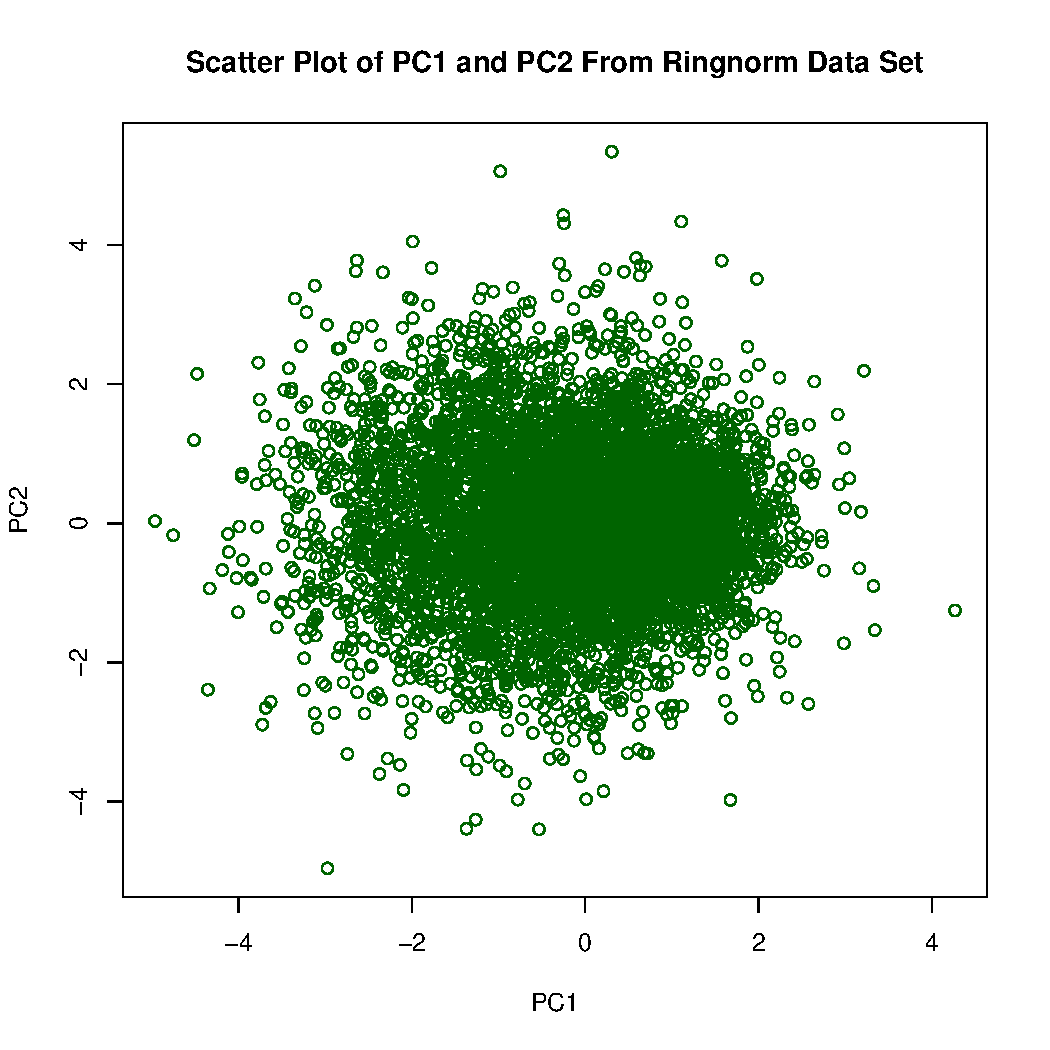
\includegraphics[width=0.7\linewidth]{Image/Prob4-1-Ringnorm.pdf}
  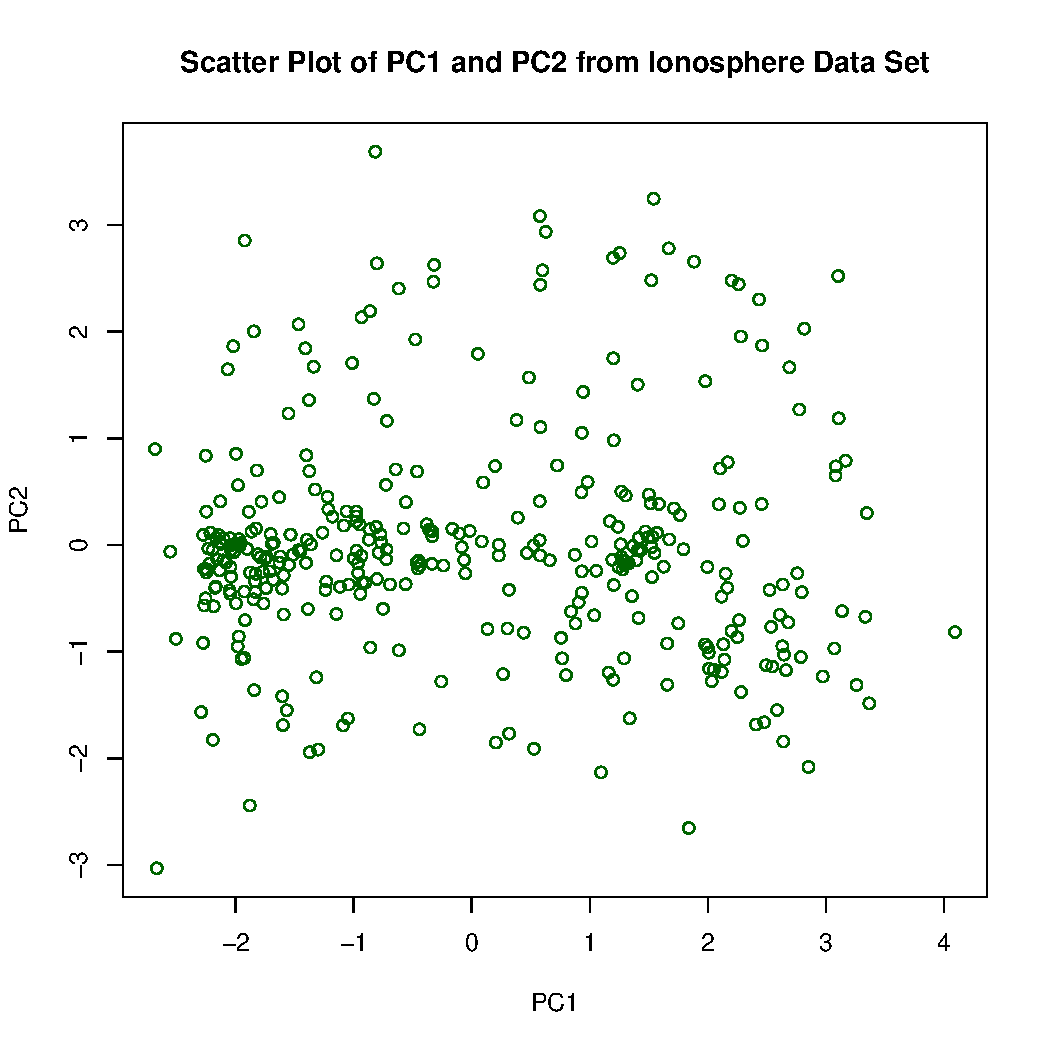
\includegraphics[width=0.7\linewidth]{Image/Prob4-1-Ionosphere.pdf}
\end{center}

By definition, PC1, or the first principal component of a set of features $X_1, X_2, \cdots, X_d$ is the normalized linear combination of the features
\[
    Z_1 = \phi_{11}X_1 + \phi_{21}X_2 + \cdots + \phi_{p1}X_d
\]
that has the largest variance. Similarly, PC2 is the linear combination
\[
    Z_2 = \phi_{12}X_1 + \phi_{22}X_2 + \cdots + \phi_{p2}X_d
\]
that has the second largest variance.
Intuitively, PC1 is the projection of data onto the direction in the data space along which the sample variance is the largest. PC2 is the projection onto the direction along which the sample variance is the second largest.


From the scatter plots of PC1 and PC2 from both data sets, we can see that PC1 and PC2 are highly uncorrelated. This is natural from method of PCA (princomp, in which eigenvector approach is used), since the eigenvectors with different eigenvalues are orthogonal vectors in $\mathbb{R}^n$. This also works for our purpose of reducing dimensions, because orthogonality, or specifically here, uncorrelation, will make sure that the space spanned by a certain number of vectors is as large as possible.
\bigskip

The actual values of PC1 and PC2 (both vectors of length $n$, where $n$ is the number of data points) are given in the R code, in \code{Prob4-1to3.R}.
\bigskip\bigskip








\qnum{4.2}
\begin{center}
  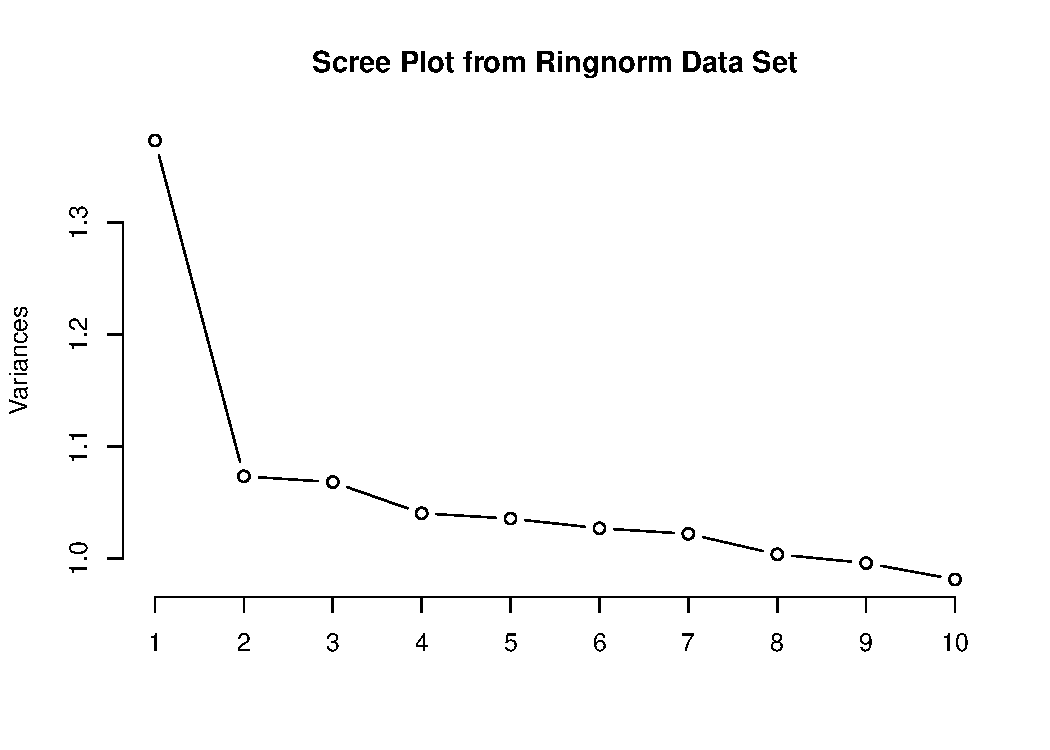
\includegraphics[width=0.7\linewidth]{Image/Prob4-2-Ringnorm1.pdf}
  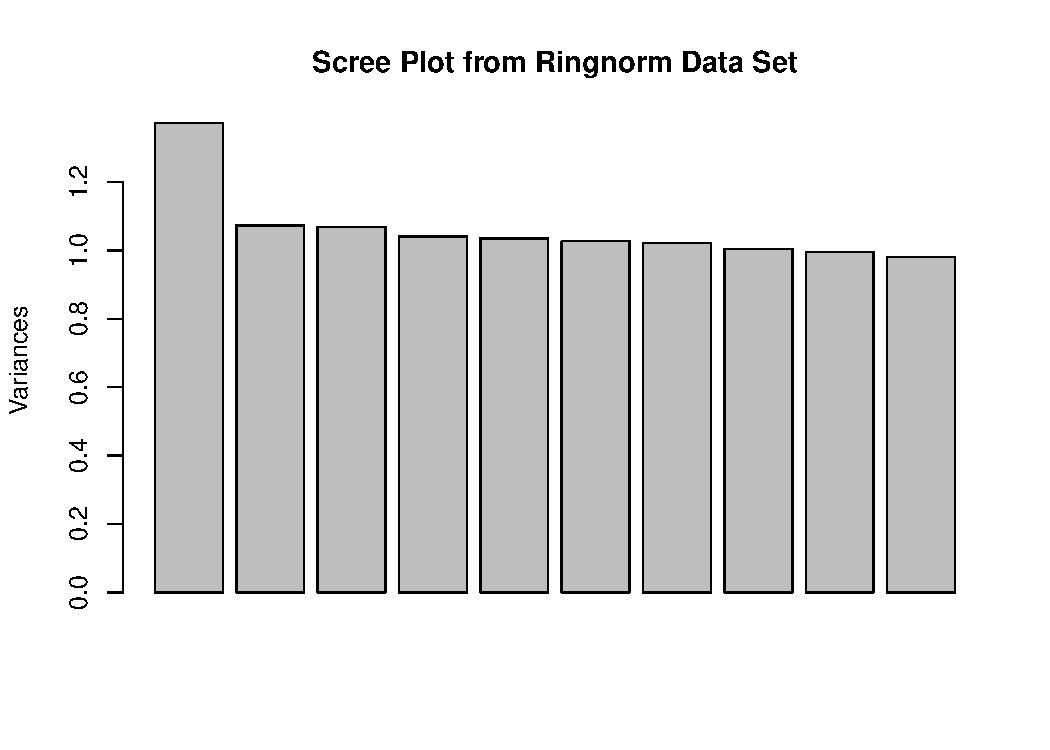
\includegraphics[width=0.7\linewidth]{Image/Prob4-2-Ringnorm2.pdf}
\end{center}


For the Ringnorm data set, we can see from the scree plots that PC1 explains most of the variances (1.37 or 6.86\%). 
Each of PC2-PC10 explains variances of around 1 or about 5\%.
\bigskip



\begin{center}
  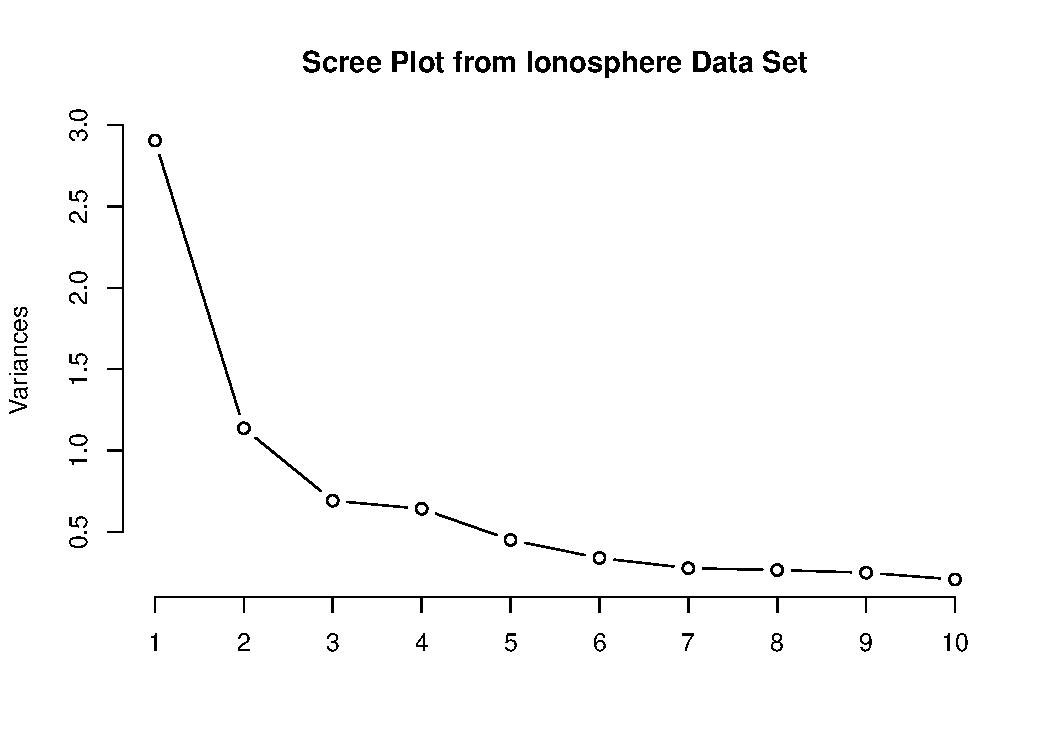
\includegraphics[width=0.7\linewidth]{Image/Prob4-2-Ionosphere1.pdf}
  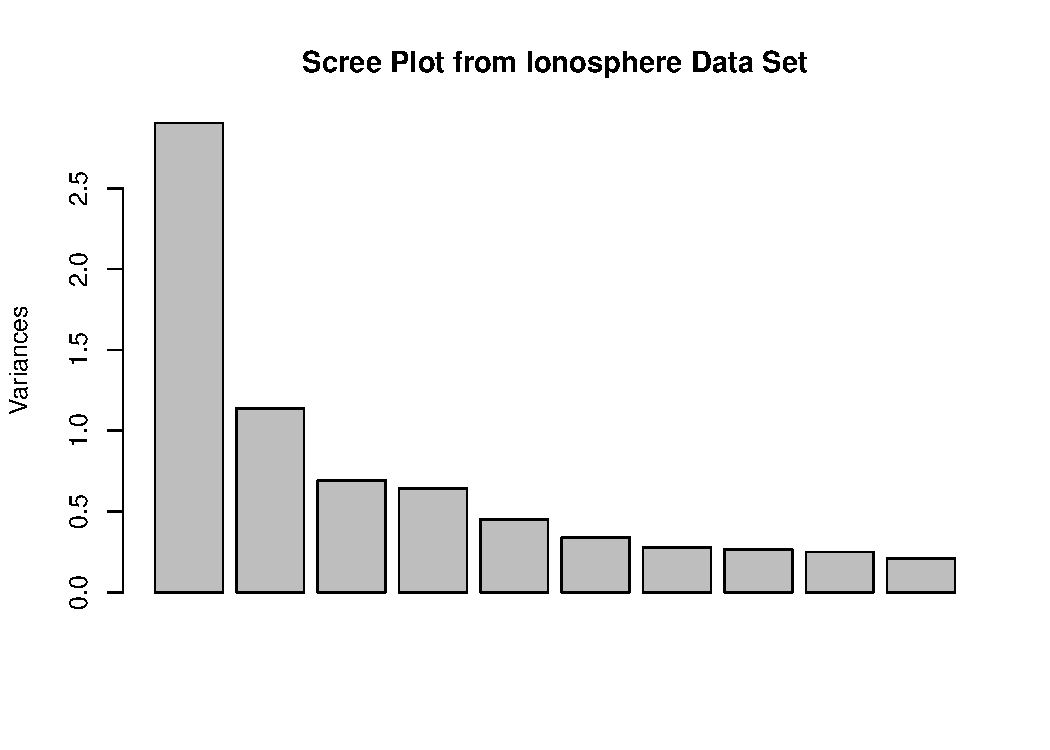
\includegraphics[width=0.7\linewidth]{Image/Prob4-2-Ionosphere2.pdf}
\end{center}
For the Ionosphere data set, we can see from the scree plots that PC1 explains most of the variances (2.90 or 31.34\%). 
PC2 explains a portion variance of 1.14 or about 12.27\%. PC3-PC4 each explain less than 10\% and PC5-PC10 each explain less than 5\% of all the variances.
\bigskip\bigskip






\qnum{4.3}
By definition, PC1, or the first principal component of a set of features $X_1, X_2, \cdots, X_d$ is the normalized linear combination of the features
\[
    Z_1 = \phi_{11}X_1 + \phi_{21}X_2 + \cdots + \phi_{p1}X_d
\]
that has the largest variance. Similarly, the $i$th principle component is the linear combination
\[
    Z_i = \phi_{1i}X_1 + \phi_{2i}X_2 + \cdots + \phi_{pi}X_d
\]
that has the $i$th largest variance. 
The $i^\text{th}$ \textbf{loading vector} is defined as the vector
\[
    \phi_i = (\phi_{1i}, \phi_{2i},\dots, \phi_{di})^T
\]
such that $Z_i$ has the $i$th largest variance. 

From a perspective of data $\textbf{X}\in \mathbb{R}^{n\times d}$, we have the following relationship:

The loading vector $\phi_k = (\phi_{1k}, \phi_{2k},\dots, \phi_{dk})^T$ is defined as the solution of 
\[
    {\arg\max}_{\phi_{1k},\cdots,\phi_{dk}}\left[
        \frac{1}{n}\sum_{i=1}^n
        \left(\sum_{j=1}^d
            \phi_{jk}x_{ij}
        \right)^2
    \right]
\]
and the $j$th component of the $k$th PC is
\[
    z_{jk} = \phi_{1k}x_{j1} + \phi_{2k}x_{j2} + \cdots + \phi_{dk}x_{jd}
\]

Intuitively, the $i$th loading vector is the direction in the data space along which the sample variance is the $i$th largest. They are the directions onto which we project our data points to get the principal components.
\bigskip\bigskip



\qnum{4.4}
\begin{center}
    \textcolor{mydarkgreen}{\textbf{Ringnorm Data Set}}
\end{center}
\bigskip

\noindent (1) Comparison between two methods:

\begin{center}
  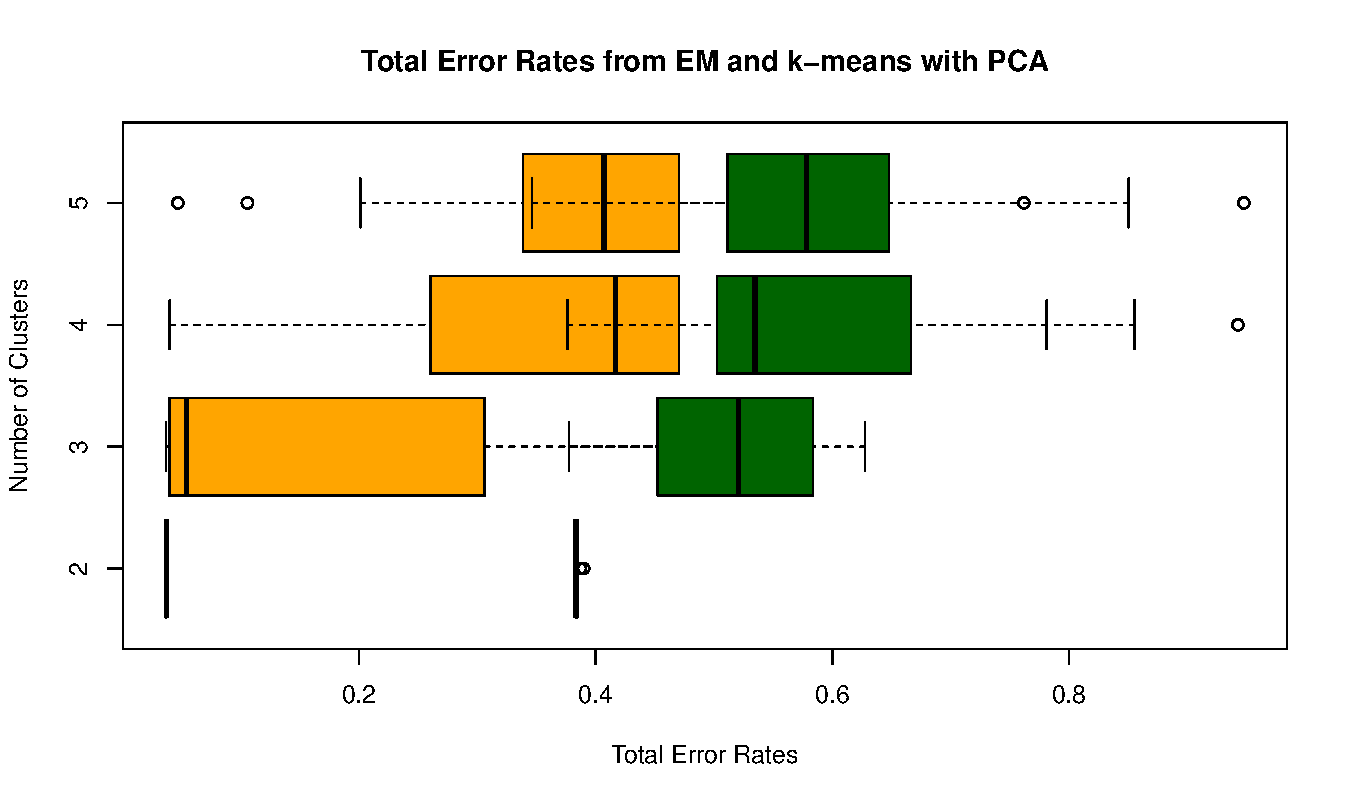
\includegraphics[width=0.9\linewidth]{Image/Prob4-4-TotalErr-Ringnorm-Both.pdf}
  
  % Comments
   \parbox{0.9\textwidth}{\textit{In the plot, the \textcolor{myorange}{orange boxes} represent total error rates from the EM algorithm, while the \textcolor{mydarkgreen}{green boxes} represent rates from the $k$-means algorithm.
  }}
\end{center}
\bigskip

\begin{center}
  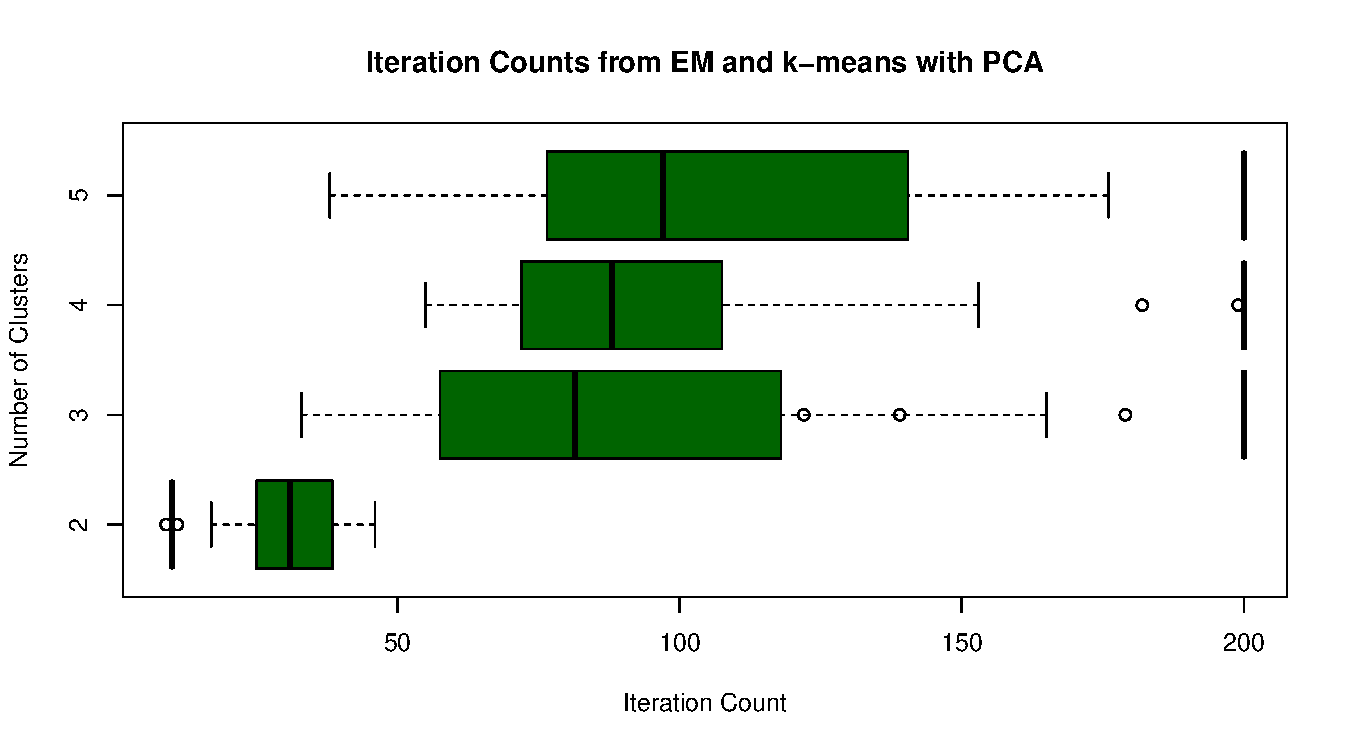
\includegraphics[width=0.9\linewidth]{Image/Prob4-4-ItrCount-Ringnorm-Both.pdf}
  
  % Comments
   \parbox{0.9\textwidth}{\textit{In the plot, the \textcolor{myorange}{orange boxes} represent iteration counts from the EM algorithm, while the \textcolor{mydarkgreen}{green boxes} represent counts from the $k$-means algorithm. 
   All algorithms had maximum iteration number capped at 200. The EM algorithm does not seem to converge well on $k = 3,\ 4,$ and $5$.
  }}
\end{center}
\bigskip

\noindent (2) EM method only:
\begin{center}
  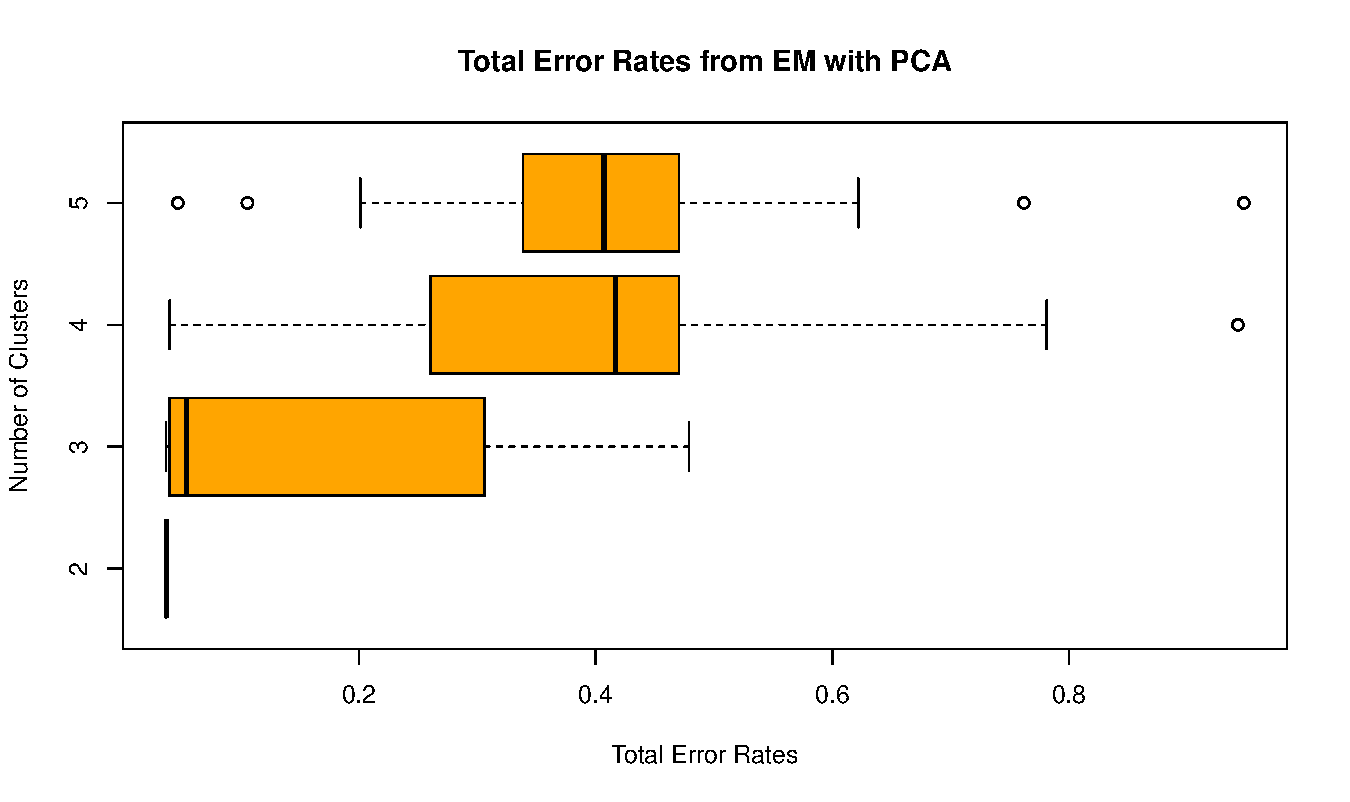
\includegraphics[width=0.8\linewidth]{Image/Prob4-4-TotalErr-Ringnorm-EMPCA.pdf}
\end{center}
\begin{center}
  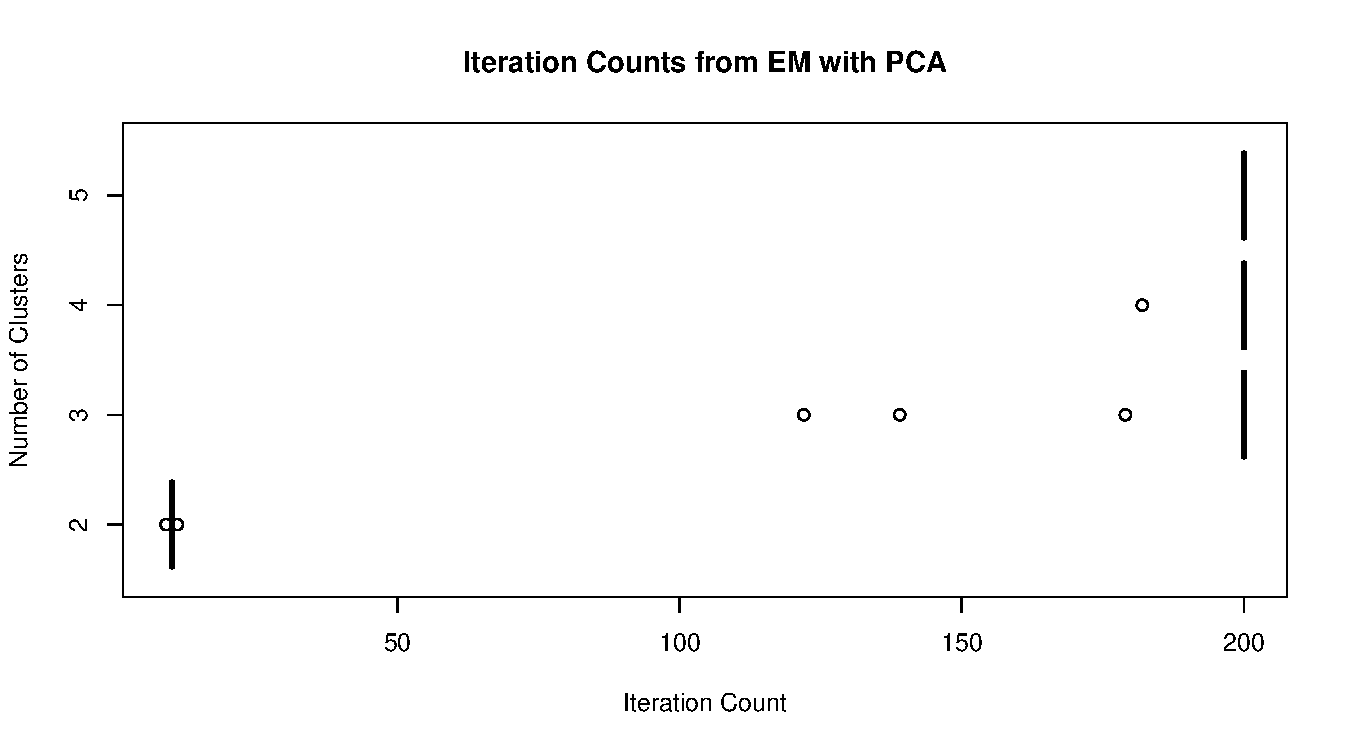
\includegraphics[width=0.8\linewidth]{Image/Prob4-4-ItrCount-Ringnorm-EMPCA.pdf}
\end{center}
\bigskip

\noindent (3) $k$-means method only:
\begin{center}
  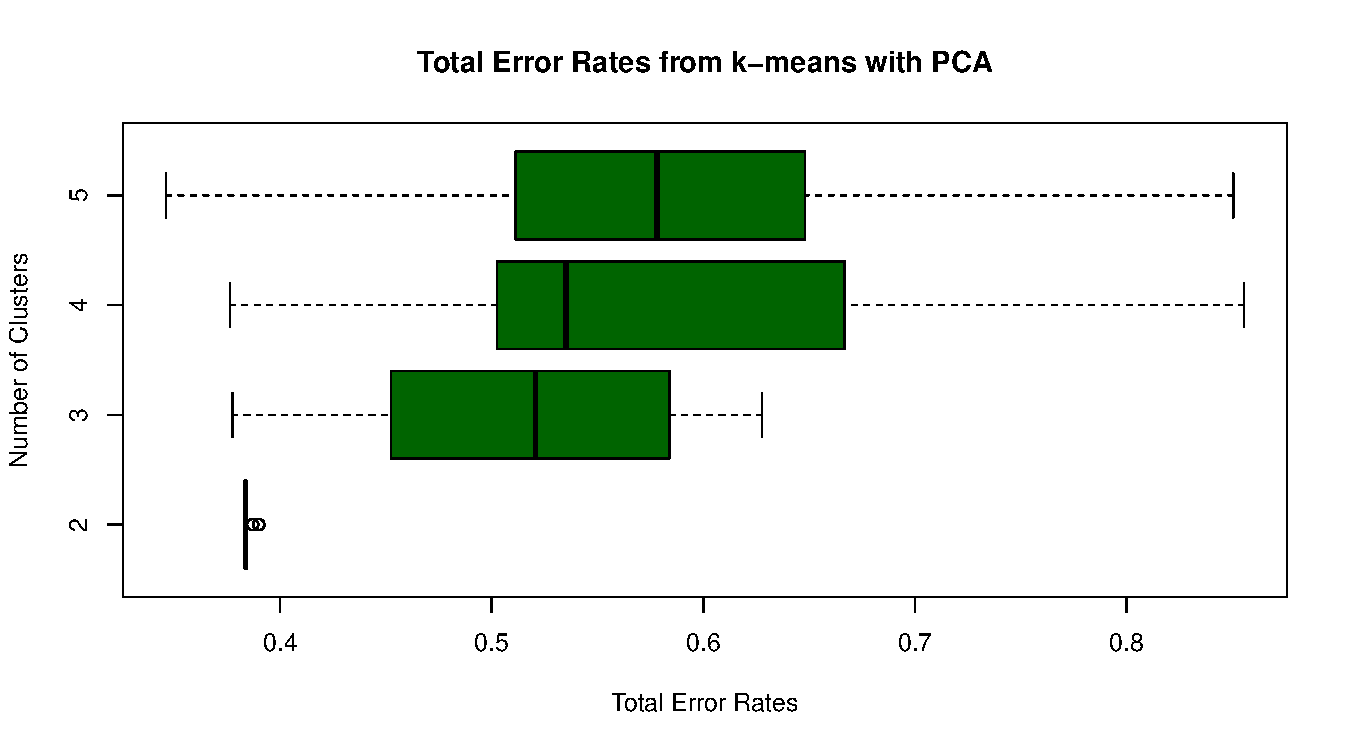
\includegraphics[width=0.8\linewidth]{Image/Prob4-4-TotalErr-Ringnorm-kmeansPCA.pdf}
\end{center}
\begin{center}
  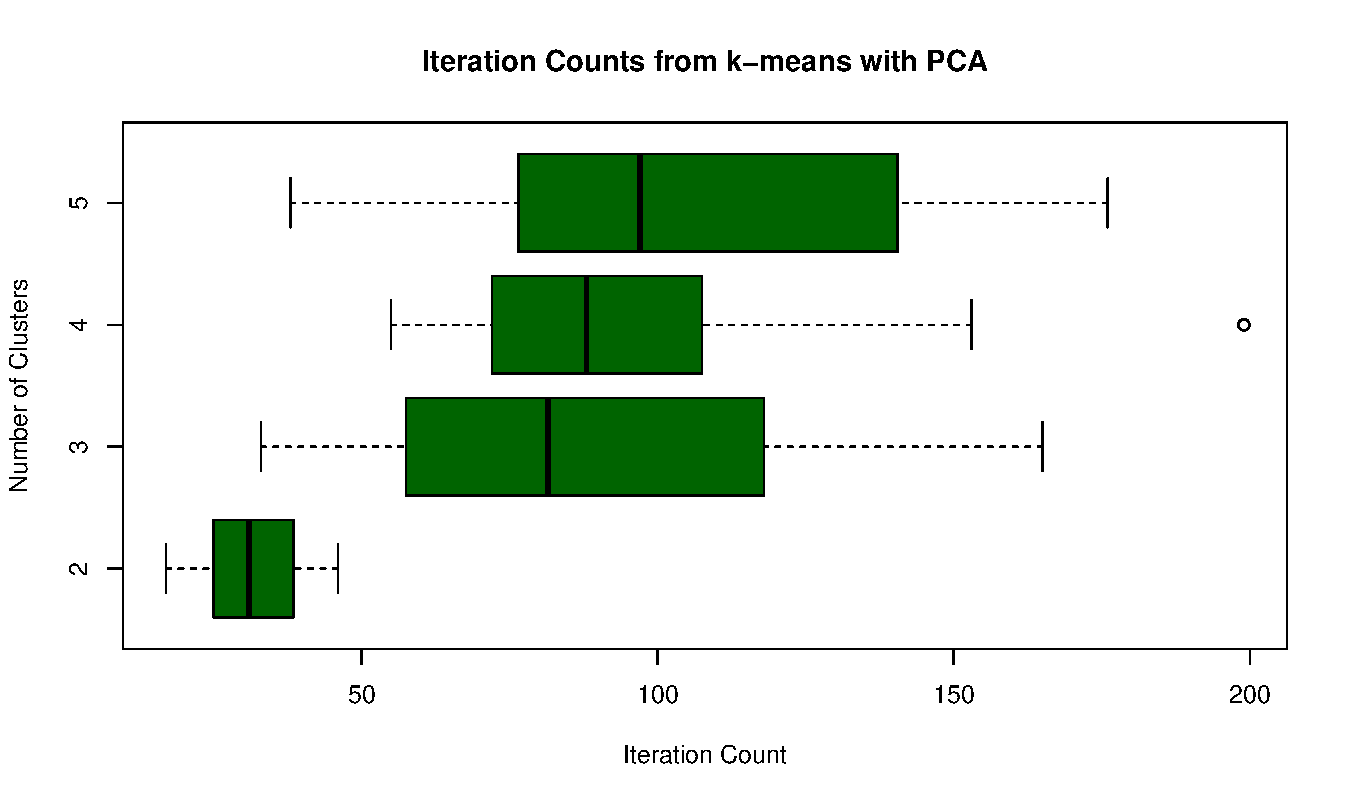
\includegraphics[width=0.8\linewidth]{Image/Prob4-4-ItrCount-Ringnorm-kmeansPCA.pdf}
\end{center}





\bigskip
\begin{center}
    \textcolor{mydarkgreen}{\textbf{Ionosphere Data Set}}
\end{center}

\noindent (1) Comparison between two methods:

\begin{center}
  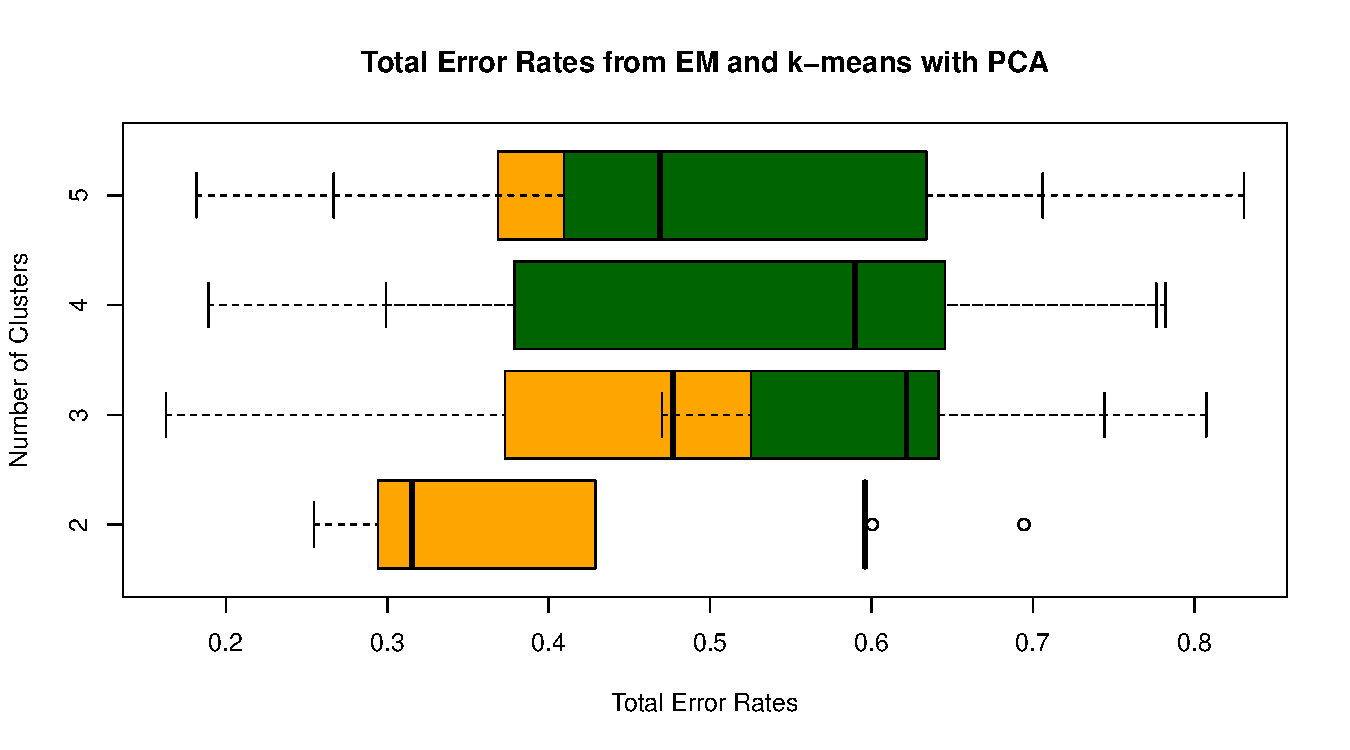
\includegraphics[width=0.9\linewidth]{Image/Prob4-4-TotalErr-Ionosphere-Both.pdf}
  
  % Comments
   \parbox{0.9\textwidth}{\textit{In the plot, the \textcolor{myorange}{orange boxes} represent total error rates from the EM algorithm, while the \textcolor{mydarkgreen}{green boxes} represent rates from the $k$-means algorithm.
  }}
\end{center}
\bigskip

\begin{center}
  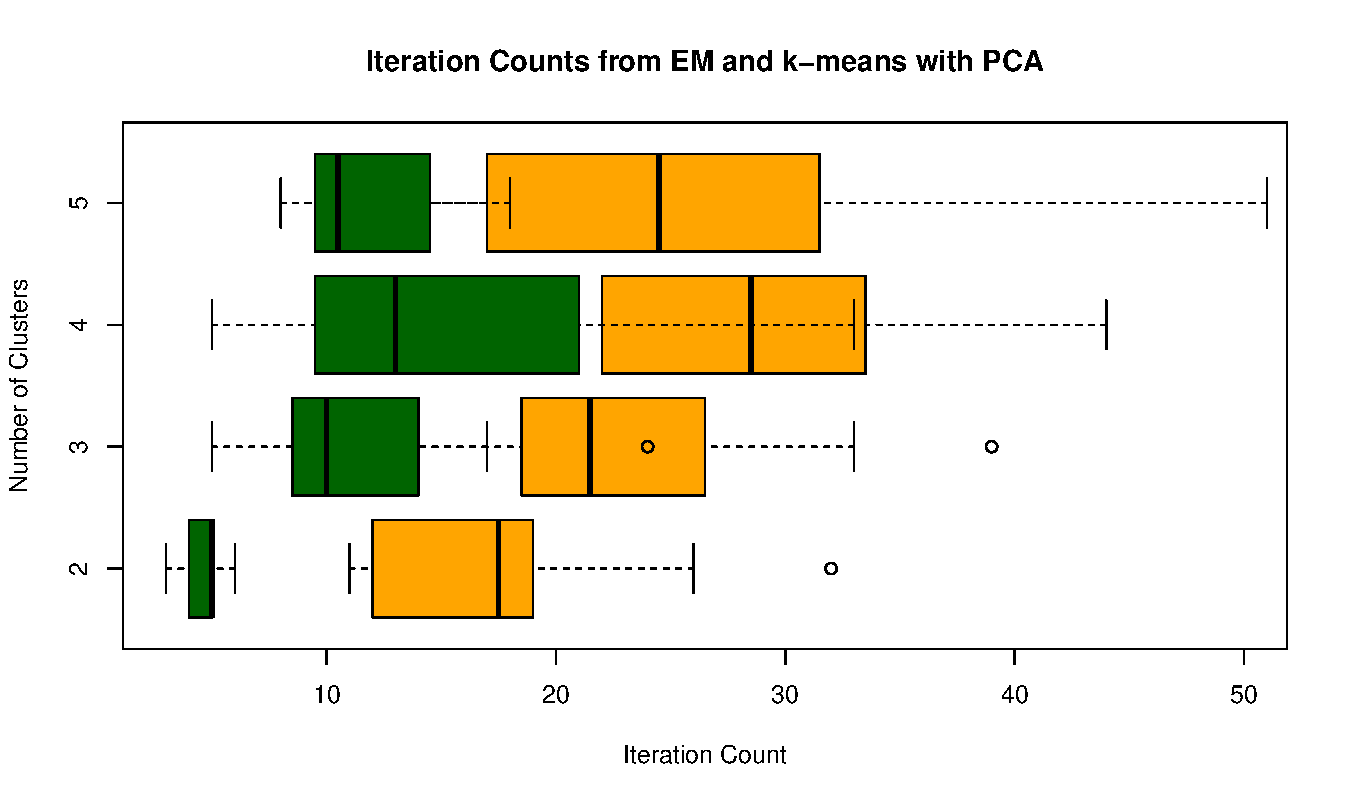
\includegraphics[width=0.9\linewidth]{Image/Prob4-4-ItrCount-Ionosphere-Both.pdf}
  
  % Comments
   \parbox{0.9\textwidth}{\textit{In the plot, the \textcolor{myorange}{orange boxes} represent iteration counts from the EM algorithm, while the \textcolor{mydarkgreen}{green boxes} represent counts from the $k$-means algorithm.  
  }}
\end{center}
\bigskip

\noindent (2) EM method only:
\begin{center}
  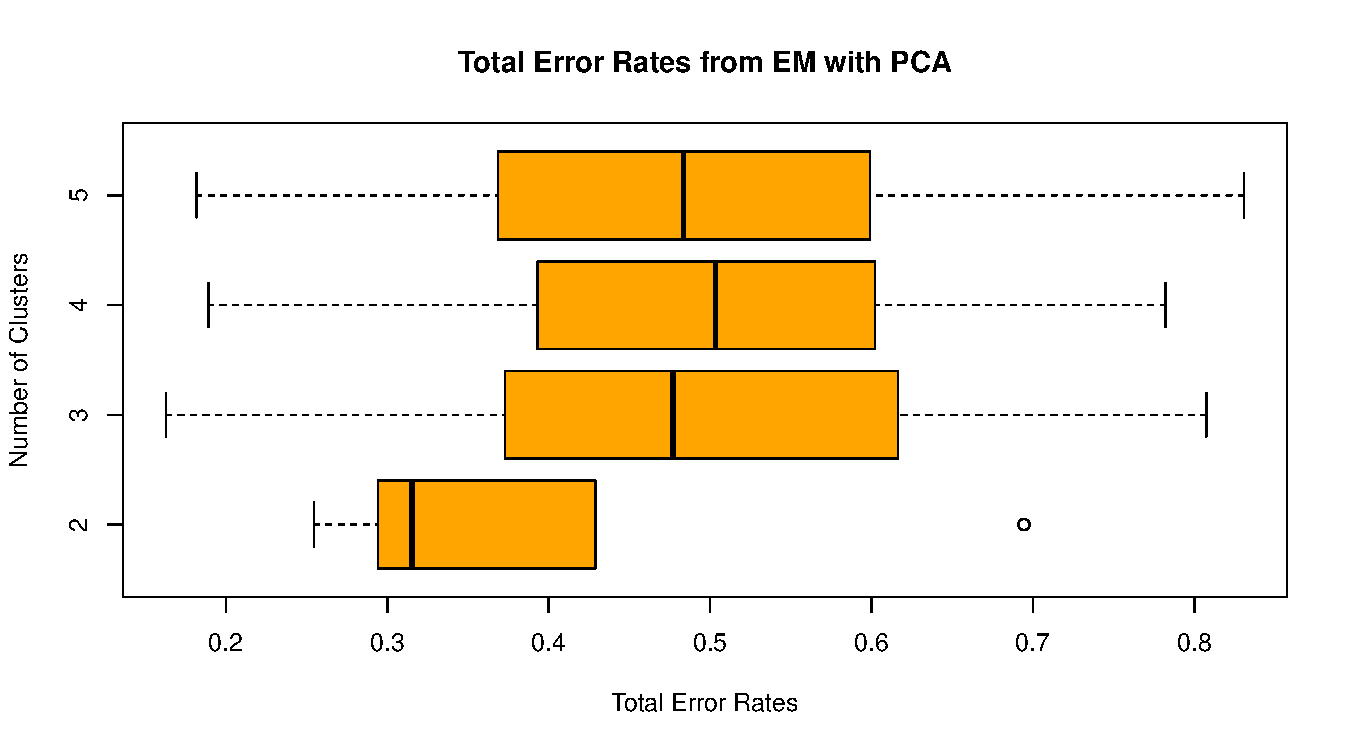
\includegraphics[width=0.8\linewidth]{Image/Prob4-4-TotalErr-Ionosphere-EMPCA.pdf}
\end{center}
\begin{center}
  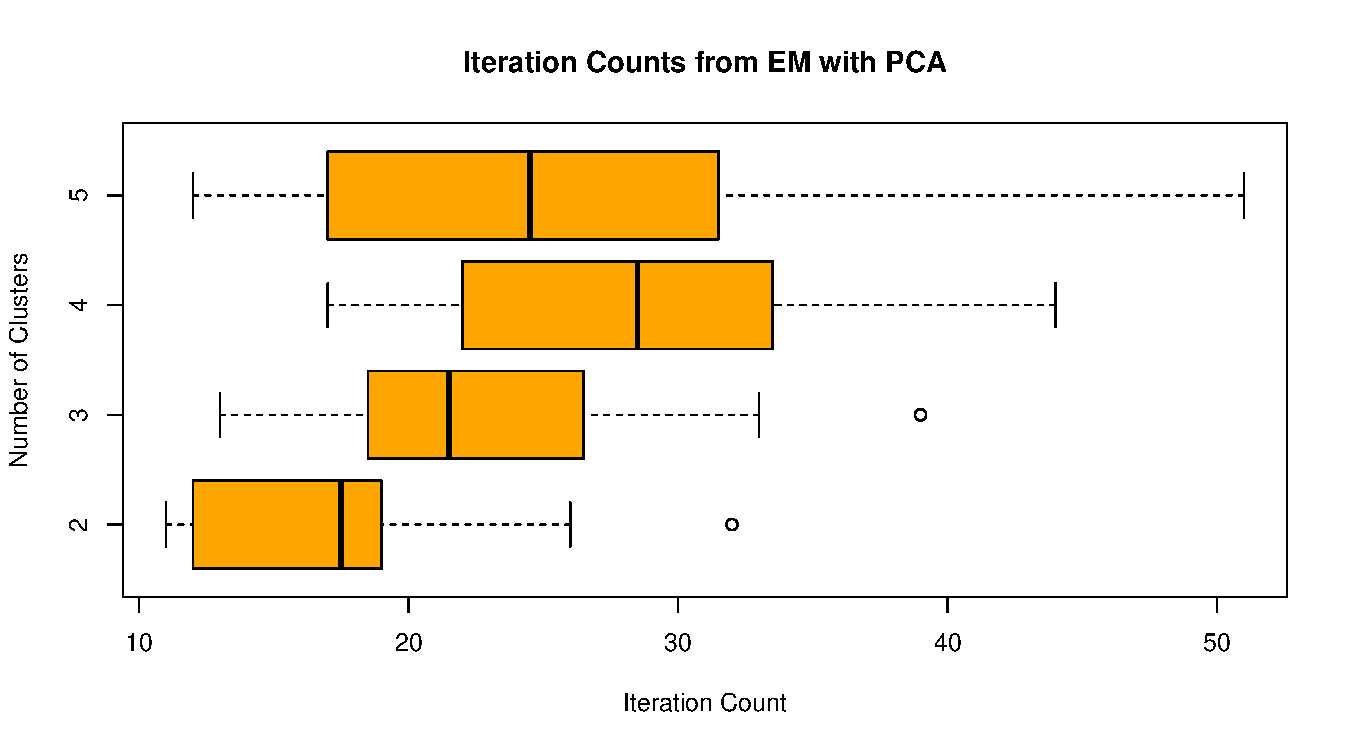
\includegraphics[width=0.8\linewidth]{Image/Prob4-4-ItrCount-Ionosphere-EMPCA.pdf}
\end{center}
\bigskip

\noindent (3) $k$-means method only:
\begin{center}
  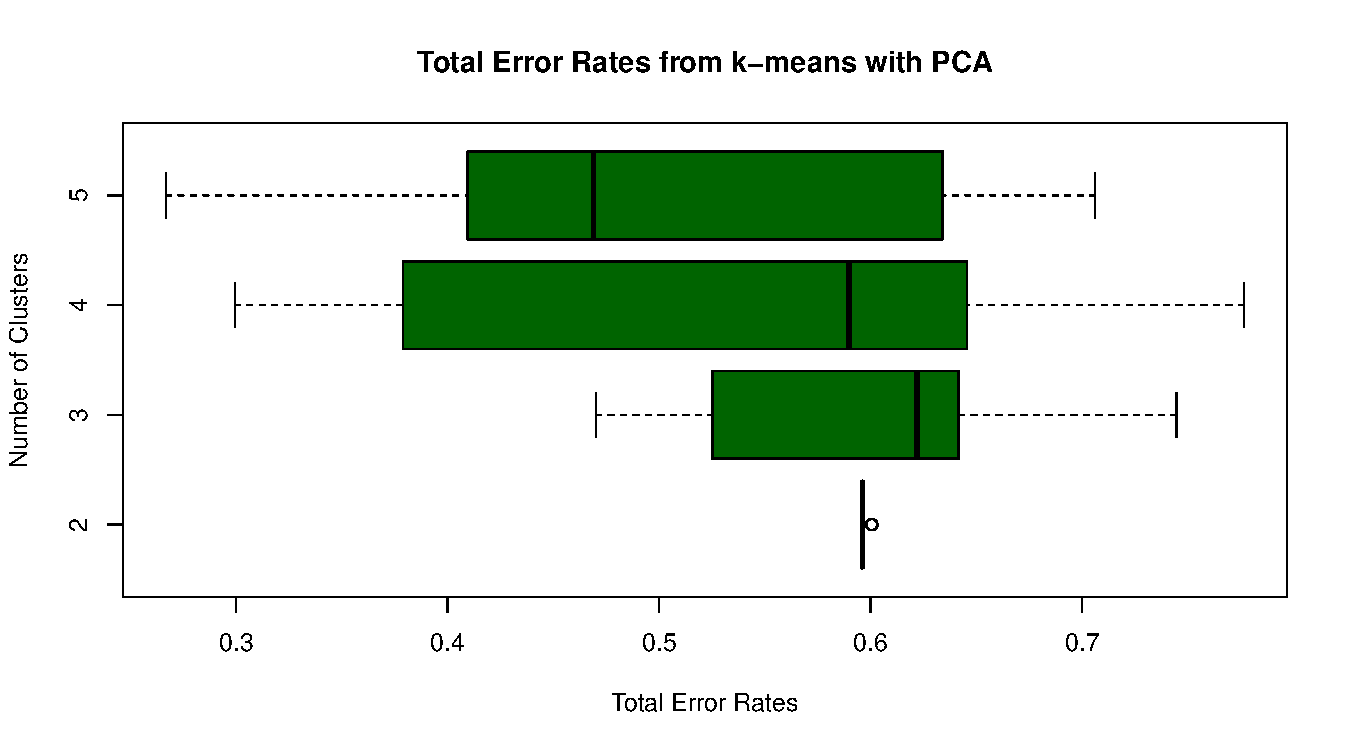
\includegraphics[width=0.8\linewidth]{Image/Prob4-4-TotalErr-Ionosphere-kmeansPCA.pdf}
\end{center}
\begin{center}
  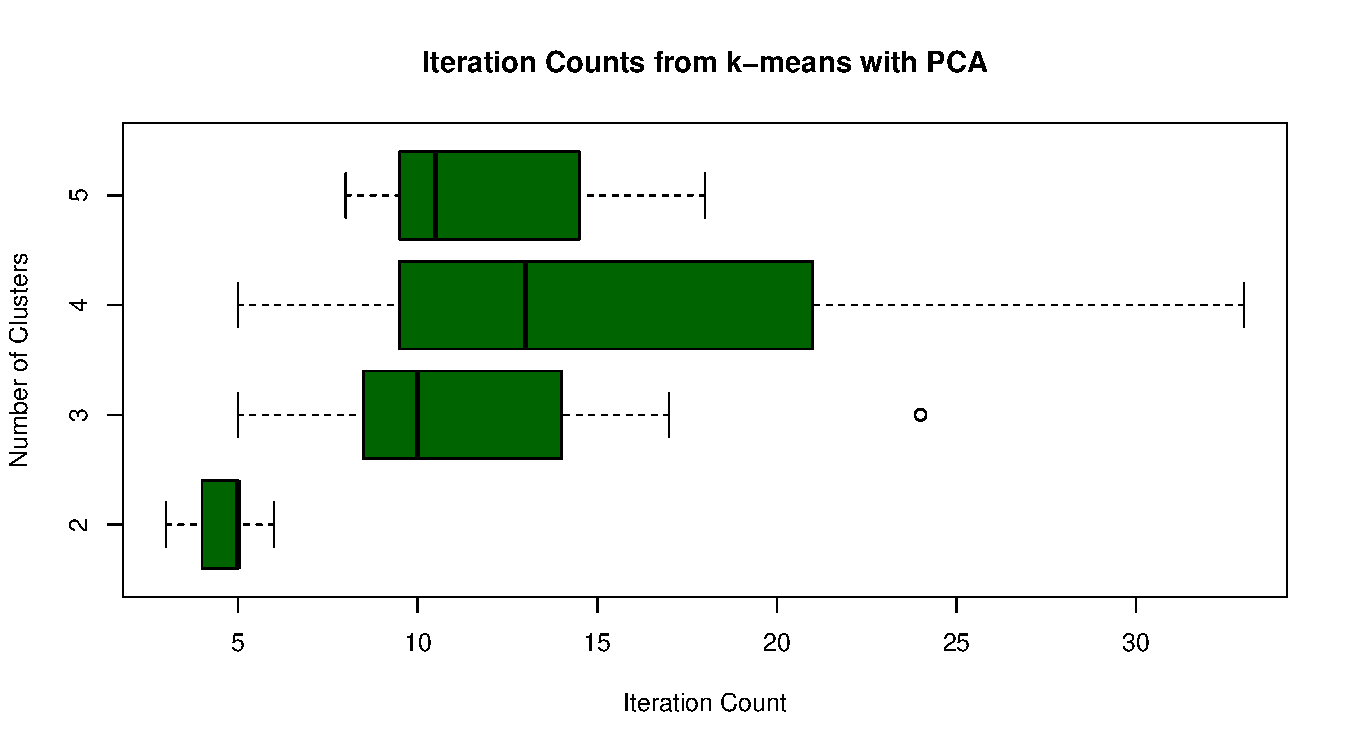
\includegraphics[width=0.8\linewidth]{Image/Prob4-4-ItrCount-Ionosphere-kmeansPCA.pdf}
\end{center}




\bigskip
\begin{center}
    \textcolor{mydarkgreen}{\textbf{Analysis of Results}}
\end{center}

\noindent 
(1) \emph{On the Ringnorm data set.}

In this data set, the EM with PCA performs significantly better on the total error rates for all $k$.

On the iteration counts, the EM algorithm works better than $k$-means when $k=2$. For $k=3,\ 4,$ and 5, the EM algorithm does not converge well. But when capped at a maximum of 200 iterations, the EM already reaches better error rates than the $k$-means.

One thing to note about the comparison of iteration counts is that, for \emph{my} implementations of the EM and $k$-means algorithms in R, this comparison does not reflect the comparison of actual run time of the two algorithms. In \emph{my} implementations, EM is much more efficient than the \km algorithm, partly due to the efficiency of matrix computations in \code{R}. This might change if the implementation changes, e.g. if the code is written in \code{C} instead. In our experiment, there is no conclusion on the actual run time of the algorithms. We can only compare the actual run time on our \code{R} implementations.
\bigskip\bigskip


\noindent 
(2) \emph{On the Ionosphere data set.}

In this data set, EM with PCA performs better on the total error rates in general. EM gives significantly lower total error rates for $k=2$. For other $k$ values, however, the EM gives better error rates but not the difference from \km is less significant.

On the iteration counts, the EM algorithm uses more iterations than $k$-means for all $k$. 

The issue on the comparison of performances mentioned in the last paragraph of (1) also applies here.
\bigskip\bigskip





\qnum{4.5}
\emph{Total error rates.}
On both the Ringnorm and the Ionosphere data sets, 
EM and $k$-means both perform worse after applying PCA and keeping 90\% of variances, resulting in an increase in the total error rates. But the results on the error rates are not different by a large scale. This is expected, as information loses after we apply PCA, which results in the increase of the error rates. But since we kept 90\% of the variances, most information is preserved, which results in a relatively small increase in the error rates.

\emph{Total Number of Iterations.} 
Before and after PCA, there is no significant change in the number of iterations in both algorithms.





























  %%%%%%%%%%%%%%%%%%%%%%%%%%%%%%%%%%%%%%%%%%%%%%%%%%%%%
%                      PROBLEM 5

 %%%%%%%%%%%%%%%%%%%%%%%%%%%%%%%%%%%%%%%%%%%%%%%%%%%%%

 \newpage
 \section*{Problem 5 [50 points]}  Randomly choose 50 points from Ionosphere data set (call this data set $\text{I}_{50}$) and perform hierarchical clustering. You are allowed to use R packages for this question. (Ignore the class variable while performing hierarchical clustering.)
 \\ 
 
 \begin{enumerate}
  \item[\textbf{5.1}]  Using hierarchical clustering with complete linkage and Euclidean distance cluster $\text{I}_{50}$. Plot the dendrogram.
\\ 
 
\item[\textbf{5.2}] Cut the dendrogram at a height that results in two distinct  clusters. Calculate an error rate.
\\  


  \item[\textbf{5.3}] First, perform PCA on $\text{I}_{50}$ (Keep $90\%$ of variance ). Then hierarchically cluster the reduced data using complete linkage and Euclidean distance. Plot the dendrogram
\\  
  
  
    \item[\textbf{5.4}]  Cut the dendrogram at a height that results in two distinct  clusters. Calculate an error rate. How  did PCA affect hierarchical clustering?
\end{enumerate}
\sep 

\qnum{5.1}
\begin{center}
  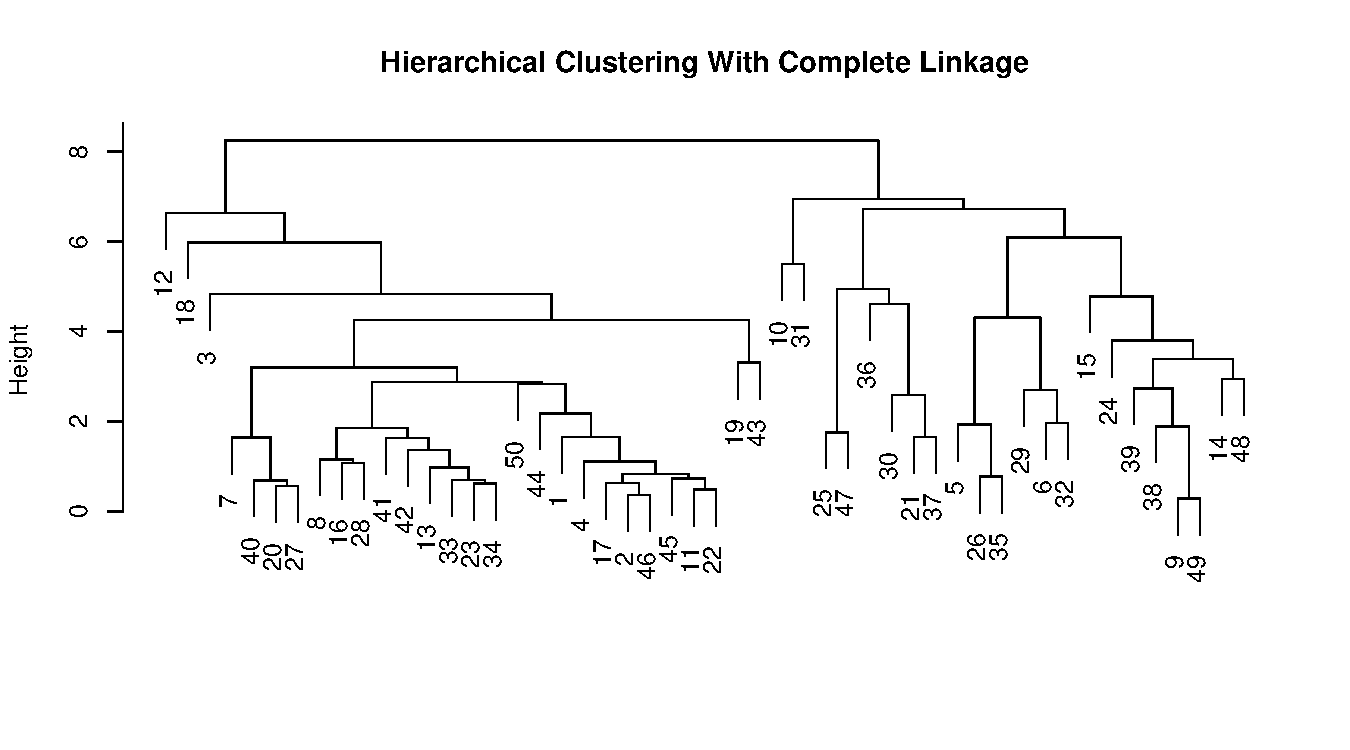
\includegraphics[width=1\linewidth]{Image/Prob5-1.pdf}
  
  \vspace{-40pt}
  \parbox{0.9\textwidth}{\textit{In the dendrogram, the number in each node correspond to the index of the data point. In the data matrix, this is the same as the row number of the data point.
  }}
\end{center}
\bigskip\bigskip

\qnum{5.2}
We cut the dendrogram at height 7 and the result is 
\begin{itemize}
    \item cluster 1 = $\{$
        1, 2, 3, 4, 7, 8, 11, 12, 13, 16, 17, 18, 19, 20, 22, 23, 27, 28, 33, 34, 40, 41, 42, 43, 44, 45, 46, 50
    $\}$
    \item cluster 2 = $\{$
        5, 6, 9, 10, 14, 15, 21, 24, 25, 26, 29, 30, 31, 32, 35, 36, 37, 38, 39, 47, 48, 49
    $\}$
\end{itemize}


The error rate is calculated as in Problem 4
\[
    \text{total error rate} = 0.9188312
\]




\qnum{5.3}
\begin{center}
  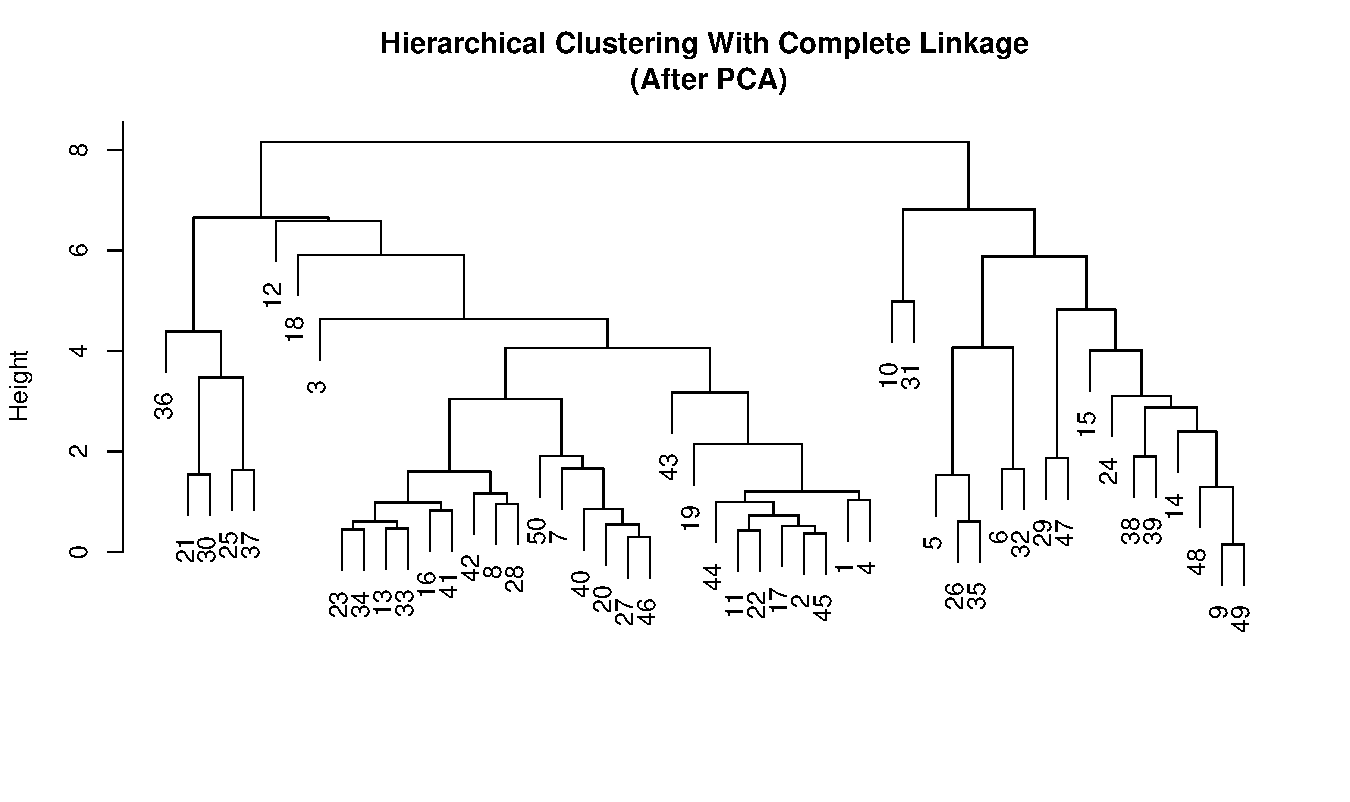
\includegraphics[width=1\linewidth]{Image/Prob5-3.pdf}
  
  \vspace{-40pt}
  \parbox{0.9\textwidth}{\textit{In the dendrogram, the number in each node correspond to the index of the data point. In the data matrix, this is the same as the row number of the data point.
  }}
\end{center}
\bigskip\bigskip


\qnum{5.4}
We cut the dendrogram at height 7 and the result is 
\begin{itemize}
    \item cluster 1 = $\{$
        1, 2, 3, 4, 7, 8, 11, 12, 13, 16, 17, 18, 19, 20, 21, 22, 23, 25, 27, 28, 30, 33, 34, 36, 37, 40, 41, 42, 43, 44, 45, 46, 50
    $\}$
    \item cluster 2 = $\{$
        5, 6, 9, 10, 14, 15, 24, 26, 29, 31, 32, 35, 38, 39, 47, 48, 49
    $\}$
\end{itemize}


The error rate is calculated as in Problem 4
\[
    \text{total error rate} = 0.9554367
\]

The results given by hierarchical cluster after PCA are slightly worse than before applying PCA. 
This is expected, as after applying PCA, we lose some of the information. And since we are keeping 90\% of the variances, the amount information lost is small, resulting in only a small increase in the total error rate.








 %%%%%%%%%%%%%%%%%%%%%%%%%%%%%%%%%%%%%%%%%%%%%%%%%%%%%

%      EXTRA CREDIT

 %%%%%%%%%%%%%%%%%%%%%%%%%%%%%%%%%%%%%%%%%%%%%%%%%%%%%
\newpage
\section*{Extra credit [60 points]}

This part is optional. 

\begin{enumerate}
\item[\textbf{1}] Improve the EM algorithm  through initialization.  \href{http://ilpubs.stanford.edu:8090/778/1/2006-13.pdf}{$k$-means ++} is an extended $k$-means clustering algorithm and induces non-uniform  distributions over  the data  that serve as  the initial centroids. Read the paper and implement this idea to improve your $G_k$ program (from question 3.1). Run your new $G_k$ and old one (question 3.1) for $k= 2,\dots,5$ and compare the results using whisker plots. [30 points]
\\

\item[\textbf{2}]  Run the EM algorithm for different mixture models, i.e., Poisson,  and against different data sets. [30 points]
\end{enumerate}
\sep 

\qnum{EC1}
\begin{center}
    \textcolor{mydarkgreen}{\textbf{Ringnorm Data Set}}
\end{center}
\bigskip

\noindent (1) Comparison between two methods:

\begin{center}
  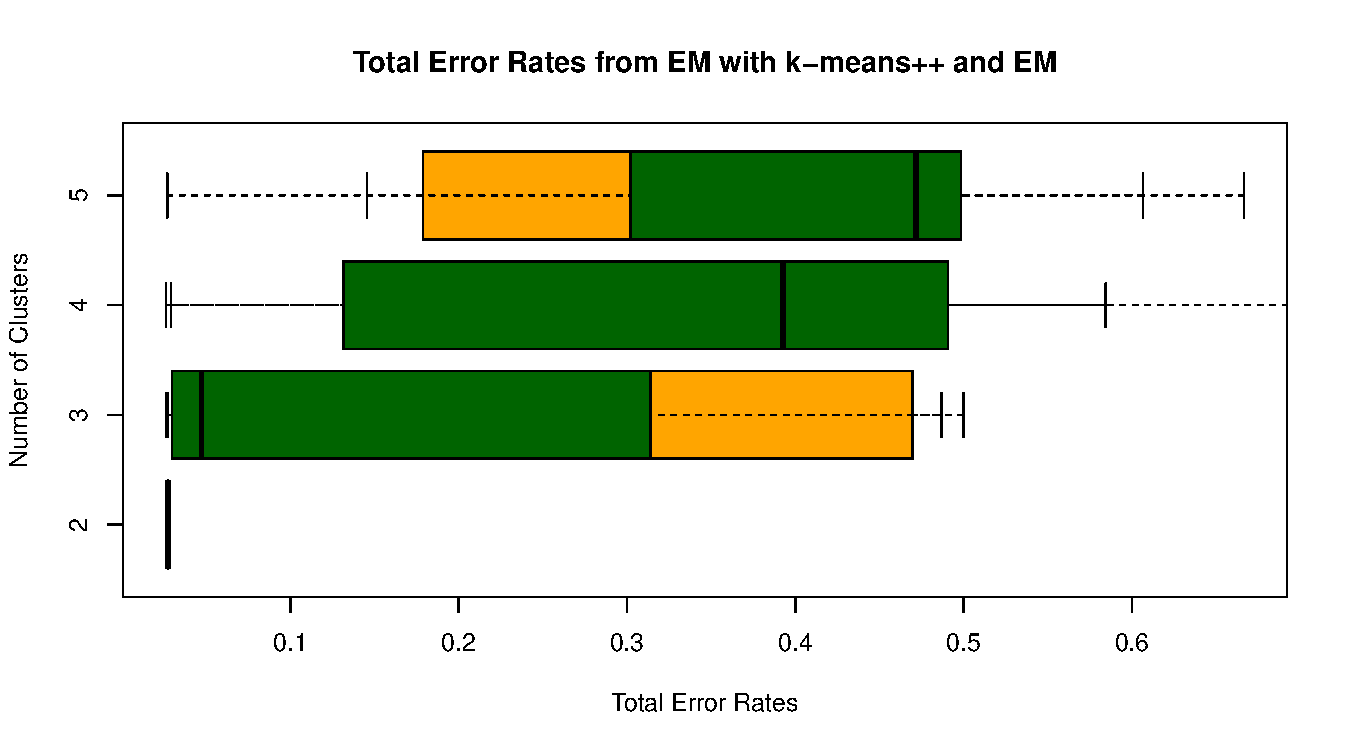
\includegraphics[width=0.9\linewidth]{Image/ProbEC1-TotalErr-Ringnorm-Both.pdf}
  
  % Comments
   \parbox{0.9\textwidth}{\textit{In the plot, the \textcolor{myorange}{orange boxes} represent total error rates from the EM algorithm with k-means++, while the \textcolor{mydarkgreen}{green boxes} represent rates from the original EM algorithm.
  }}
\end{center}
\bigskip

\begin{center}
  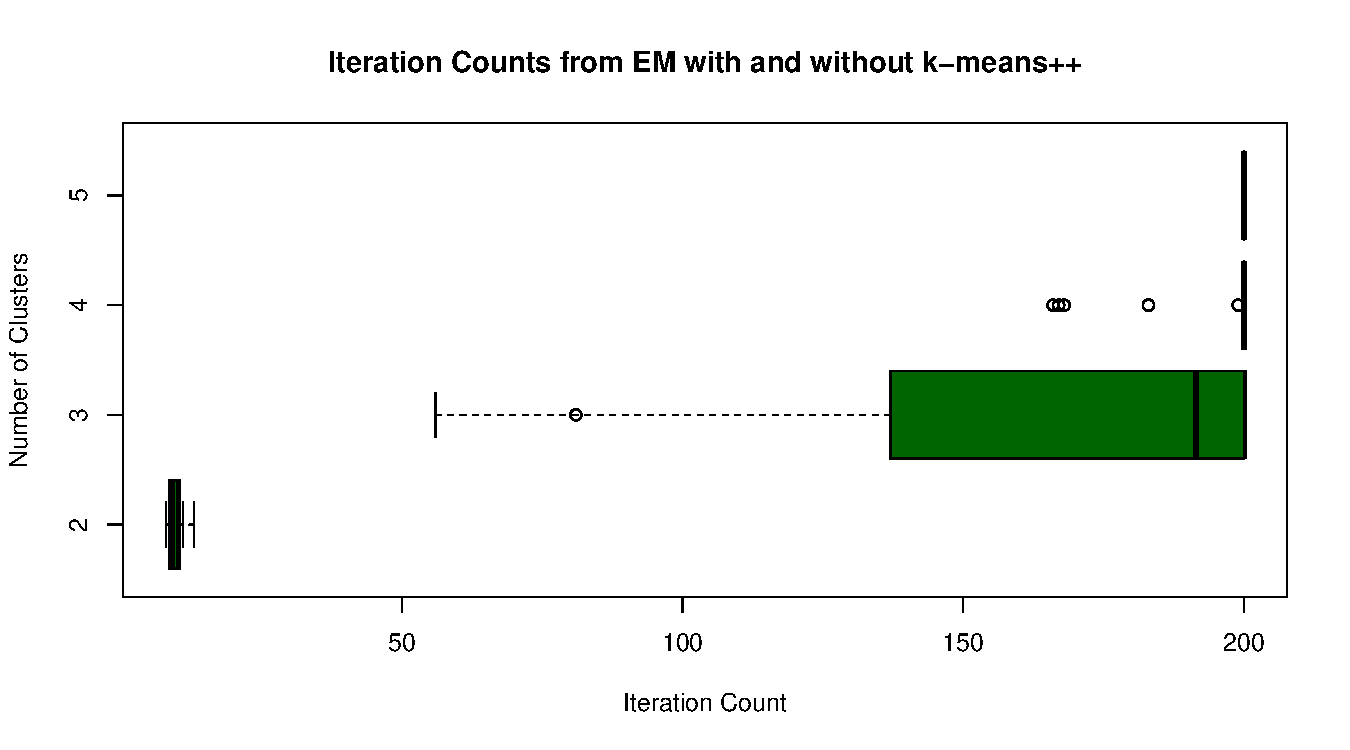
\includegraphics[width=0.9\linewidth]{Image/ProbEC1-ItrCount-Ringnorm-Both.pdf}
  
  % Comments
   \parbox{0.9\textwidth}{\textit{In the plot, the \textcolor{myorange}{orange boxes} represent iteration counts from the EM algorithm with k-means++, while the \textcolor{mydarkgreen}{green boxes} represent counts from the original EM algorithm algorithm. 
   All algorithms had maximum iteration number capped at 200.
  }}
\end{center}
\bigskip

\noindent (2) EM method with \km++ only:
\begin{center}
  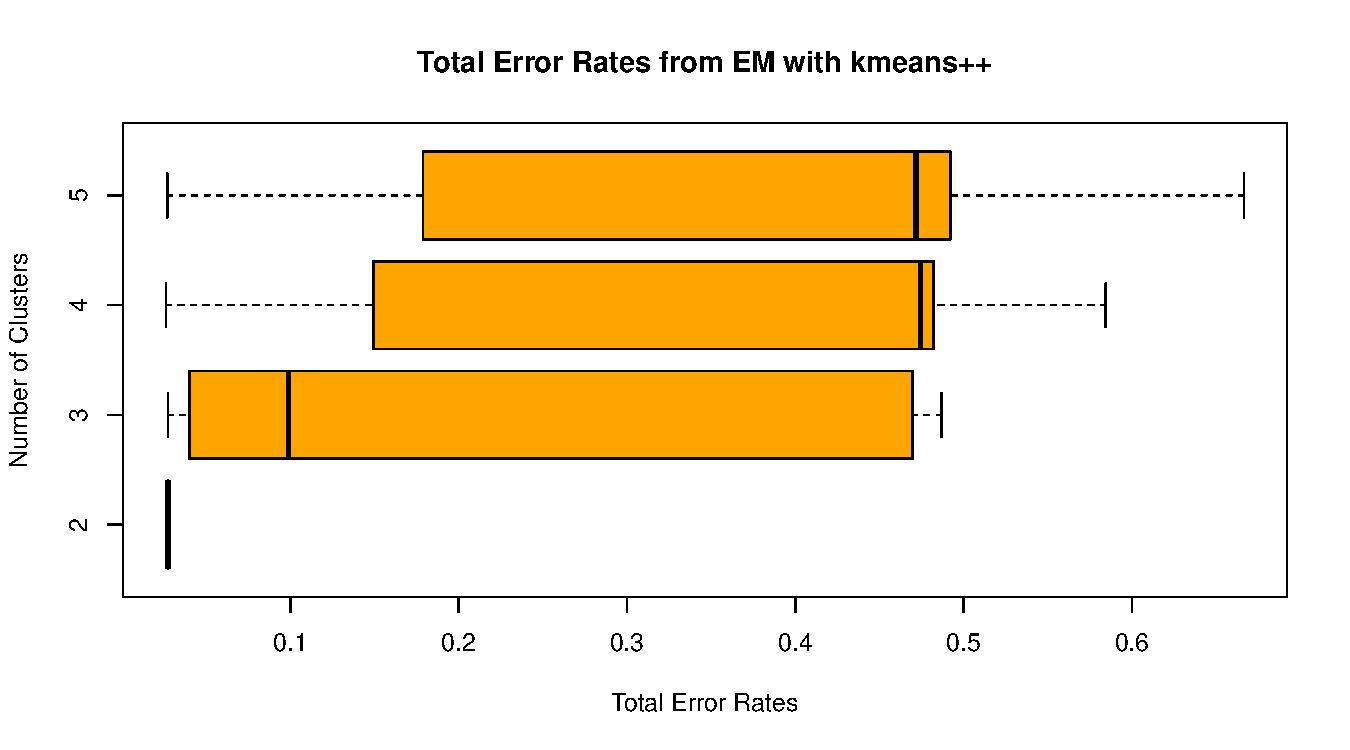
\includegraphics[width=0.8\linewidth]{Image/ProbEC1-TotalErr-Ringnorm-EMkpp.pdf}
\end{center}
\begin{center}
  \includegraphics[width=0.8\linewidth]{Image/ProbEC1-ItrCount-Ringnorm-EMkpp.pdf}
\end{center}
\bigskip

\noindent (3) Original EM method only:
\begin{center}
  \includegraphics[width=0.8\linewidth]{Image/ProbEC1-TotalErr-Ringnorm-EM.pdf}
\end{center}
\begin{center}
  \includegraphics[width=0.8\linewidth]{Image/ProbEC1-ItrCount-Ringnorm-EM.pdf}
\end{center}







\bigskip
\begin{center}
    \textcolor{mydarkgreen}{\textbf{Ionosphere Data Set}}
\end{center}

\noindent (1) Comparison between two methods:

\begin{center}
  \includegraphics[width=0.9\linewidth]{Image/ProbEC1-TotalErr-Ionosphere-Both.pdf}
  
  % Comments
   \parbox{0.9\textwidth}{\textit{In the plot, the \textcolor{myorange}{orange boxes} represent total error rates from the EM algorithm with \km, while the \textcolor{mydarkgreen}{green boxes} represent rates from the original EM algorithm.
  }}
\end{center}
\bigskip

\begin{center}
  \includegraphics[width=0.9\linewidth]{Image/ProbEC1-ItrCount-Ionosphere-Both.pdf}
  
  % Comments
   \parbox{0.9\textwidth}{\textit{In the plot, the \textcolor{myorange}{orange boxes} represent iteration counts from the EM algorithm with \km++, while the \textcolor{mydarkgreen}{green boxes} represent counts from the original EM algorithm. 
  }}
\end{center}
\bigskip

\noindent (2) EM method with \km++ only:
\begin{center}
  \includegraphics[width=0.8\linewidth]{Image/ProbEC1-TotalErr-Ionosphere-EMkpp.pdf}
\end{center}
\begin{center}
  \includegraphics[width=0.8\linewidth]{Image/ProbEC1-ItrCount-Ionosphere-EMkpp.pdf}
\end{center}
\bigskip

\noindent (3) Original EM method only:
\begin{center}
  \includegraphics[width=0.8\linewidth]{Image/ProbEC1-TotalErr-Ionosphere-EM.pdf}
\end{center}
\begin{center}
  \includegraphics[width=0.8\linewidth]{Image/ProbEC1-ItrCount-Ionosphere-EM.pdf}
\end{center}




\bigskip
\begin{center}
    \textcolor{mydarkgreen}{\textbf{Analysis of Results}}
\end{center}

\noindent 
(1) \emph{On the Ringnorm data set.}

In this data set, the EMs with and without $k$-means++  perform similarly on both the total error rates and iteration counts for all $k$.
\bigskip


\noindent 
(2) \emph{On the Ionosphere data set.}

In this data set, the original EM performs consistently better on the total error rates in general. 

On the iteration counts, the original EM algorithm performs better in general than EM with $k$-means++ as well.
\bigskip

\noindent
(3) The slight decrease in performance may be because the initialization of $k$-means++ uses the Euclidean distance to calculate the sampling distribution, which might be compatible with the EM algorithm.
\bigskip\bigskip








\qnum{EC2}
The program is given in \code{ProbEC2-EM-SingleRun.R}. The program is tested on several random 2D sets generated from Poisson distributions with mean $\lambda = 1$. Here, we give the results from 3 of such experiments. 
Note that in the plot, the 2 clusters are separated by different colors and the circles represent data points (200 points in each experiment). Many points overlap, since Poisson distribution is discrete. The two dots represents the predicted centers of the clusters.


\begin{center}
  \includegraphics[width=0.6\linewidth]{Image/ProbEC2-1.pdf}
  
 \small{\textit{Experiment 1}}
\end{center}


\begin{center}
  \includegraphics[width=0.6\linewidth]{Image/ProbEC2-2.pdf}
  
  \small\textit{Experiment 2}
\end{center}


\begin{center}
  \includegraphics[width=0.6\linewidth]{Image/ProbEC2-3.pdf}
  
  \small\textit{Experiment 3}
\end{center}














%%%%%%%%%%%%%%%%%%%%%%%%%%%%%%%%%%%%%%%%%%%%%%%%%%%%%


%%%%%%%%%%%%%%%%%%%%%%%%%%%%%%%%%%%%%%%%%%%%%%%%%%%%%
\end{document}


